%\documentclass{sig-alternate-10pt}
%  \pdfpagewidth=8.5truein
% \pdfpageheight=11truein

\documentclass{sig-alternate-10pt}
\paperwidth=8.5in
\paperheight=11in
\usepackage[margin=1in]{geometry}

\usepackage{cite}
\usepackage{epsfig,endnotes}
\usepackage{fancyhdr}
\usepackage{rotating}
\usepackage[tight,footnotesize]{subfigure}
\usepackage{graphicx}
\usepackage{amssymb}
\usepackage{amsmath}
\usepackage{url}
\usepackage{multicol}
\usepackage{epsf,psfrag}
\usepackage{indentfirst}
\usepackage{float}
\usepackage{color}
\newcommand{\red}[1]{\textcolor{red}{#1}}
\newcommand{\blue}[1]{\textcolor{blue}{#1}}
\newcommand{\green}[1]{\textcolor{green}{#1}}

%\pagestyle{empty}
\begin{document}
\makeatletter
\def\@copyrightspace{\relax}
\makeatother
\pagestyle{empty}

\title{How Connected are the ACM SIG Communities?}
\numberofauthors{3} %  in this sample file, there are a *total*
\author{
\alignauthor Fabricio Benevenuto\\
       \affaddr{Universidade Federal de \\Minas Gerais, Brazil}\\
       \email{fabricio@dcc.ufmg.br}
\alignauthor Alberto H. F. Laender\\
       \affaddr{Universidade Federal de \\Minas Gerais, Brazil}\\
       \email{laender@dcc.ufmg.br}
\alignauthor Bruno L. Alves\\
       \affaddr{Universidade Federal de \\Minas Gerais, Brazil}\\
       \email{bruno.leite@dcc.ufmg.br}
}


\maketitle
\begin{abstract}
Currently, computer scientists publish more in conferences than journals and several conferences are the main venue in many computer science subareas. There has been considerable debate about the role of conferences for computer science research and one of the main arguments in favor of them is that conferences bring researchers together, allowing them to enhance collaborations and establish research communities in a young and fast-evolving discipline. In this work, we investigate if computer science conferences are really able to create collaborative research communities by analyzing the structure of the communities formed by the flagship conferences of several ACM SIGs. Our findings show that most of these flagship conferences are able to connect their main authors in large and well-structured communities. However, we have noted that in a few ACM SIG flagship conferences authors do not collaborate over the years, creating a structure with several small disconnected components.
\end{abstract}


\section{Introduction}


There is a long debate about the role of conference publications in computer science~\cite{Fortnow:cacm2009,Patterson:cacm2004,Vardi:cacm2009,Vardi:cacm2010,Vardi:cacm2014}. On one hand, some researchers argue that conferences offer a fast and regular venue for publication of research results at the same time that allow researchers to interact with each other. These interactions would be the key for the development of research communities in a relatively young and fast-evolving discipline. On the other hand, there exists some criticism to the conference system due to the short time given to review the papers, the limited size of the papers, the review overload faced by program committee members, and the limited time for authors to revise their papers after receiving the reviews.

Despite the existing concerns on this controversial is\-sue, conferences are quite important today as computer scientists give a huge value to them~\cite{Franceschet:cacm2010,Freyne:cacm2010,Laender:sigcse2008}. Particularly, the flagship conferences of the ACM Special Interest Groups (SIGs) are often the most prestigious ones, usually being listed among the most important venues of several computer science subareas.

Although the importance of the main ACM SIG conferences to their respective research fields is incontestable, part of the argument in favor of conferences is that they help create and maintain an active research community, by simply offering a place for researchers to meet regularly and promote collaborations. In this work, we aim at investigating two questions related to this context: (1) \textit{How structured are the ACM SIG conference communities?} and (2) \textit{Who are the individuals responsible for connecting each ACM SIG conference community?}

Our effort to answer the first question consists in analyzing the coauthorship graph structure of the communities formed by the flagship conferences of the ACM SIGs. Our findings show that most of the ACM SIG conferences are able to connect their main authors in large and well-structured connected components of a coauthorship network and only very few conferences, such as the ACM Symposium on Applied Computing, flagship conference of SIGAPP, and the ACM Conference on Design of Communications, flagship conference of SIGDOC, do not form the typical structure of a research community, presenting a set of small and disconnected components.




\begin{table*}[t]
\centering
\caption{DBLP statistics for the flagship conferences of the ACM SIGs}
\begin{scriptsize}
\begin{tabular}{|l|l|c|c|c|c|c|c|c|c|} \hline
\bf{SIG} & \bf{Acronym} & \bf{Period} & \bf{Authors} & \bf{Publications} & \bf{Editions} & \bf{Aut/Edi} & \bf{Pub/Edi} & \bf{Aut/Pub}\\ \hline
SIGACT & STOC & 1969-2012 & 2159 & 2685 & 44 & 49.07 & 61.02 & 0.80\\ \hline
SIGAPP & SAC & 1993-2011 & 9146 & 4500 & 19 & 481.37 & 236.84 & 2.03\\ \hline
SIGARCH & ISCA & 1976-2011 & 2461 & 1352 & 36 & 68.36 & 37.56 & 1.82\\ \hline
SIGBED & HSCC & 1998-2012 & 846 & 617 & 15 & 56.40 & 41.13 & 1.37\\ \hline
SIGCHI & CHI & 1994-2012 & 5095 & 2819 & 19 & 268.16 & 148.37 & 1.81\\ \hline
SIGCOMM & SIGCOMM & 1988-2011 & 1593 & 796 & 24 & 66.38 & 33.17 & 2.00\\ \hline
SIGCSE & SIGCSE & 1986-2012 & 3923 & 2801 & 27 & 145.30 & 103.74 & 1.40\\ \hline
SIGDA & DAC & 1964-2011 & 8876 & 5693 & 48 & 184.92 & 118.60 & 1.56\\ \hline
SIGDOC & SIGDOC & 1989-2010 & 1071 & 810 & 22 & 48.68 & 36.82 & 1.32\\ \hline
SIGGRAPH & SIGGRAPH & 1985-2003 & 1920 & 1108 & 19 & 101.05 & 58.32 & 1.73\\ \hline
SIGIR & SIGIR & 1978-2011 & 3624 & 2687 & 34 & 106.59 & 79.03 & 1.35\\ \hline
SIGKDD & KDD & 1995-2011 & 3078 & 1699 & 17 & 181.06 & 99.94 & 1.81\\ \hline
SIGMETRICS & SIGMETRICS & 1981-2011 & 2083 & 1174 & 31 & 67.19 & 37.87 & 1.77\\ \hline
SIGMICRO & MICRO & 1987-2011 & 1557 & 855 & 25 & 62.28 & 34.20 & 1.82\\ \hline
SIGMM & MM & 1993-2011 & 5400 & 2928 & 19 & 284.21 & 154.11 & 1.84\\ \hline
SIGMOBILE & MOBICOM & 1995-2011 & 1151 & 480 & 17 & 67.71 & 28.24 & 2.40\\ \hline
SIGMOD & SIGMOD & 1975-2012 & 4202 & 2669 & 38 & 110.58 & 70.24 & 1.57\\ \hline
SIGOPS & PODC & 1982-2011 & 1685 & 1403 & 30 & 56.17 & 46.77 & 1.20\\ \hline
SIGPLAN & POPL & 1975-2012 & 1527 & 1217 & 38 & 40.18 & 32.03 & 1.25\\ \hline
SIGSAC & CCS & 1996-2011 & 1354 & 676 & 16 & 84.63 & 42.25 & 2.00\\ \hline
SIGSAM & ISSAC & 1988-2011 & 1100 & 1177 & 24 & 45.83 & 49.04 & 0.93\\ \hline
SIGSOFT & ICSE & 1987-2011 & 3502 & 2248 & 25 & 140.08 & 89.92 & 1.56\\ \hline
SIGUCCS & SIGUCCS & 1989-2011 & 1771 & 1593 & 23 & 77.00 & 69.26 & 1.11\\ \hline
SIGWEB & CIKM & 1992-2011 & 4978 & 2623 & 20 & 248.90 & 131.15 & 1.90\\ \hline
\end{tabular}
\end{scriptsize}
\label{tab:sigs_conference_period}
\end{table*}


To approach our second question, we present a tool that allows one to visualize research communities formed by authors from specific ACM SIG conferences, making it possible to identify the most prolific authors with a high level of participation in a given community. To do that, we use data from DBLP\footnote{http://dblp.uni-trier.de} and Google Scholar\footnote{scholar.google.com} to construct scientific communities and identify their leaders. Our visualization tool also allows a plethora of interesting observations about the authors as we shall see later.


The rest of this paper is organized as follows. Next section introduces the ACM SIG communities we have considered. Then, we characterize the structure of ACM SIG communities and analyze the role of their leaders. Finally,  we conclude by summarizing our results.




\section{ACM SIG Communities}

In order to construct scientific communities from ACM SIG conferences, we have gathered data from DBLP~\cite{Ley:2002,Ley:2009}, a digital library containing more than 3 million publications from more than 1.5 million authors that provides bibliographic information on major computer science conference proceedings and journals. DBLP offers its entire database in XML format, which facilitates gathering the data and constructing entire scientific communities.

Each publication is accompanied by its title, list of authors, year of publication, and publication venue, i.e., conference or journal. For the purpose of our work, we consider a research network as a coauthorship graph in which nodes represent authors (researchers) and edges link coauthors of papers published in conferences that put together specific research communities~\cite{Alves:2013}. In order to define such communities, we focus on the publications from the flagship conferences of major ACM SIGs. Thus, we define a scientific community by linking researchers that have coauthored a paper in a certain conference, making the ACM SIG flagship conferences to act as communities in which coauthorships are formed.

In total, 24 scientific communities have been constructed. Table~\ref{tab:sigs_conference_period} lists these communities, including the respective ACM SIG, the conference acronym, the period considered (some conferences had their period reduced to avoid hiatus in the data), the total number of authors, publications and editions as well as ratios extracted from these last three figures. We make this dataset available for the research community.
For more details, we refer the reader to our previous efforts that use it~\cite{Alves:2013,benevenuto2015hindexparadox}.


\section{Structure of the ACM SIG \\ Communities}

%girvan2002community
%A community in a graph is usually defined as a set nodes densely connected that are sparsely connected to other nodes in the graph~\cite{girvan2002community}.
%There are various algorithms and strategies to identify communities in a graph.

Ideally, it is expected that over the years conferences are able to bring together researchers with common interests so that they can collaborate to advance a certain field. Thus, it is expected that with a few decades, the coauthorship graph of a certain community contains a largest connected component (LCC)~\cite{newman2010networks} that puts together a large part (i.e., the majority) of its authors. In other words, one could expect a large LCC in a research community in which authors often interact and collaborate, meaning that there exists at least one path among a large fraction of them.

Table~\ref{tab:largestSCC} shows the percentage of the authors of each community that are part of the largest connected component of its respective coauthorship graph. Clearly, we can note that most of the research communities formed by SIG conferences have a large connected component that is typically larger than half of the network, suggesting that these conferences have successfully put together their researchers in a collaborative network. Figure~\ref{fig:redes_top} depicts the networks of the three conferences with the most representative largest connected components, SIGMOD, STOC and CHI, and the three conferences with the least representative ones, SIGUCCS, SAC and SIGDOC. In these networks, connected components are shown with different colours and the LCC is presented as the most central one. The size of each node represents an estimative of the importance of a researcher to the scientific community, which is discussed in the next section. As we can see, the latter are the only three communities that are formed by a very small largest connected component (i.e., with less than 10\% of the researchers in the network) and several other small connected components. Typically, these conferences cover a wide range of topics, making it difficult for their researchers to establish a research community. For example, SAC is an annual conference organized in technical tracks that change at each edition. Although this dynamic format attracts a large number of submissions every year, it does not contribute to the formation of a specific, well-structured research community.


\begin{table}[!htbp]
\caption{Structure of the scientific communities}
\centering
\begin{scriptsize}
\begin{tabular}{|l|c|} \hline
\textbf{Conference} & \textbf{Largest Connected Component}  \\ \hline
SIGMOD & 74.75\%  \\ \hline
STOC & 74.34\% \\ \hline
CHI & 73.33\%  \\ \hline
MICRO & 65.13\%  \\ \hline
HSCC & 62.53\%  \\ \hline
DAC & 62.21\%  \\ \hline
KDD & 61.24\% \\ \hline
ISCA & 58.72\% \\ \hline
SIGCOMM & 57.88\%  \\ \hline
SIGIR & 57.86\%  \\ \hline
SIGCSE & 55.31\%  \\ \hline
ICSE & 52.68\%  \\ \hline
PODC & 52.46\% \\ \hline
CIKM & 51.81\%  \\ \hline
CCS & 51.70\%  \\ \hline
SIGMETRICS & 50.89\%  \\ \hline
POPL & 50.82\%  \\ \hline
MM & 50.06\% \\ \hline
SIGGRAPH & 46.72\%  \\ \hline
ISSAC & 44.09\% \\ \hline
MOBICOM & 37.88\%  \\ \hline
SIGDOC & 9.69\% \\ \hline
SAC & 3.67\% \\ \hline
SIGUCCS & 3.27\% \\ \hline
\end{tabular}
\end{scriptsize}
\label{tab:largestSCC}
\end{table}



\begin{figure*}[!htb]
  \begin{center}
  \subfigure[SIGMOD (74.75\%)]{
    \label{fig:rede_sigmod}
    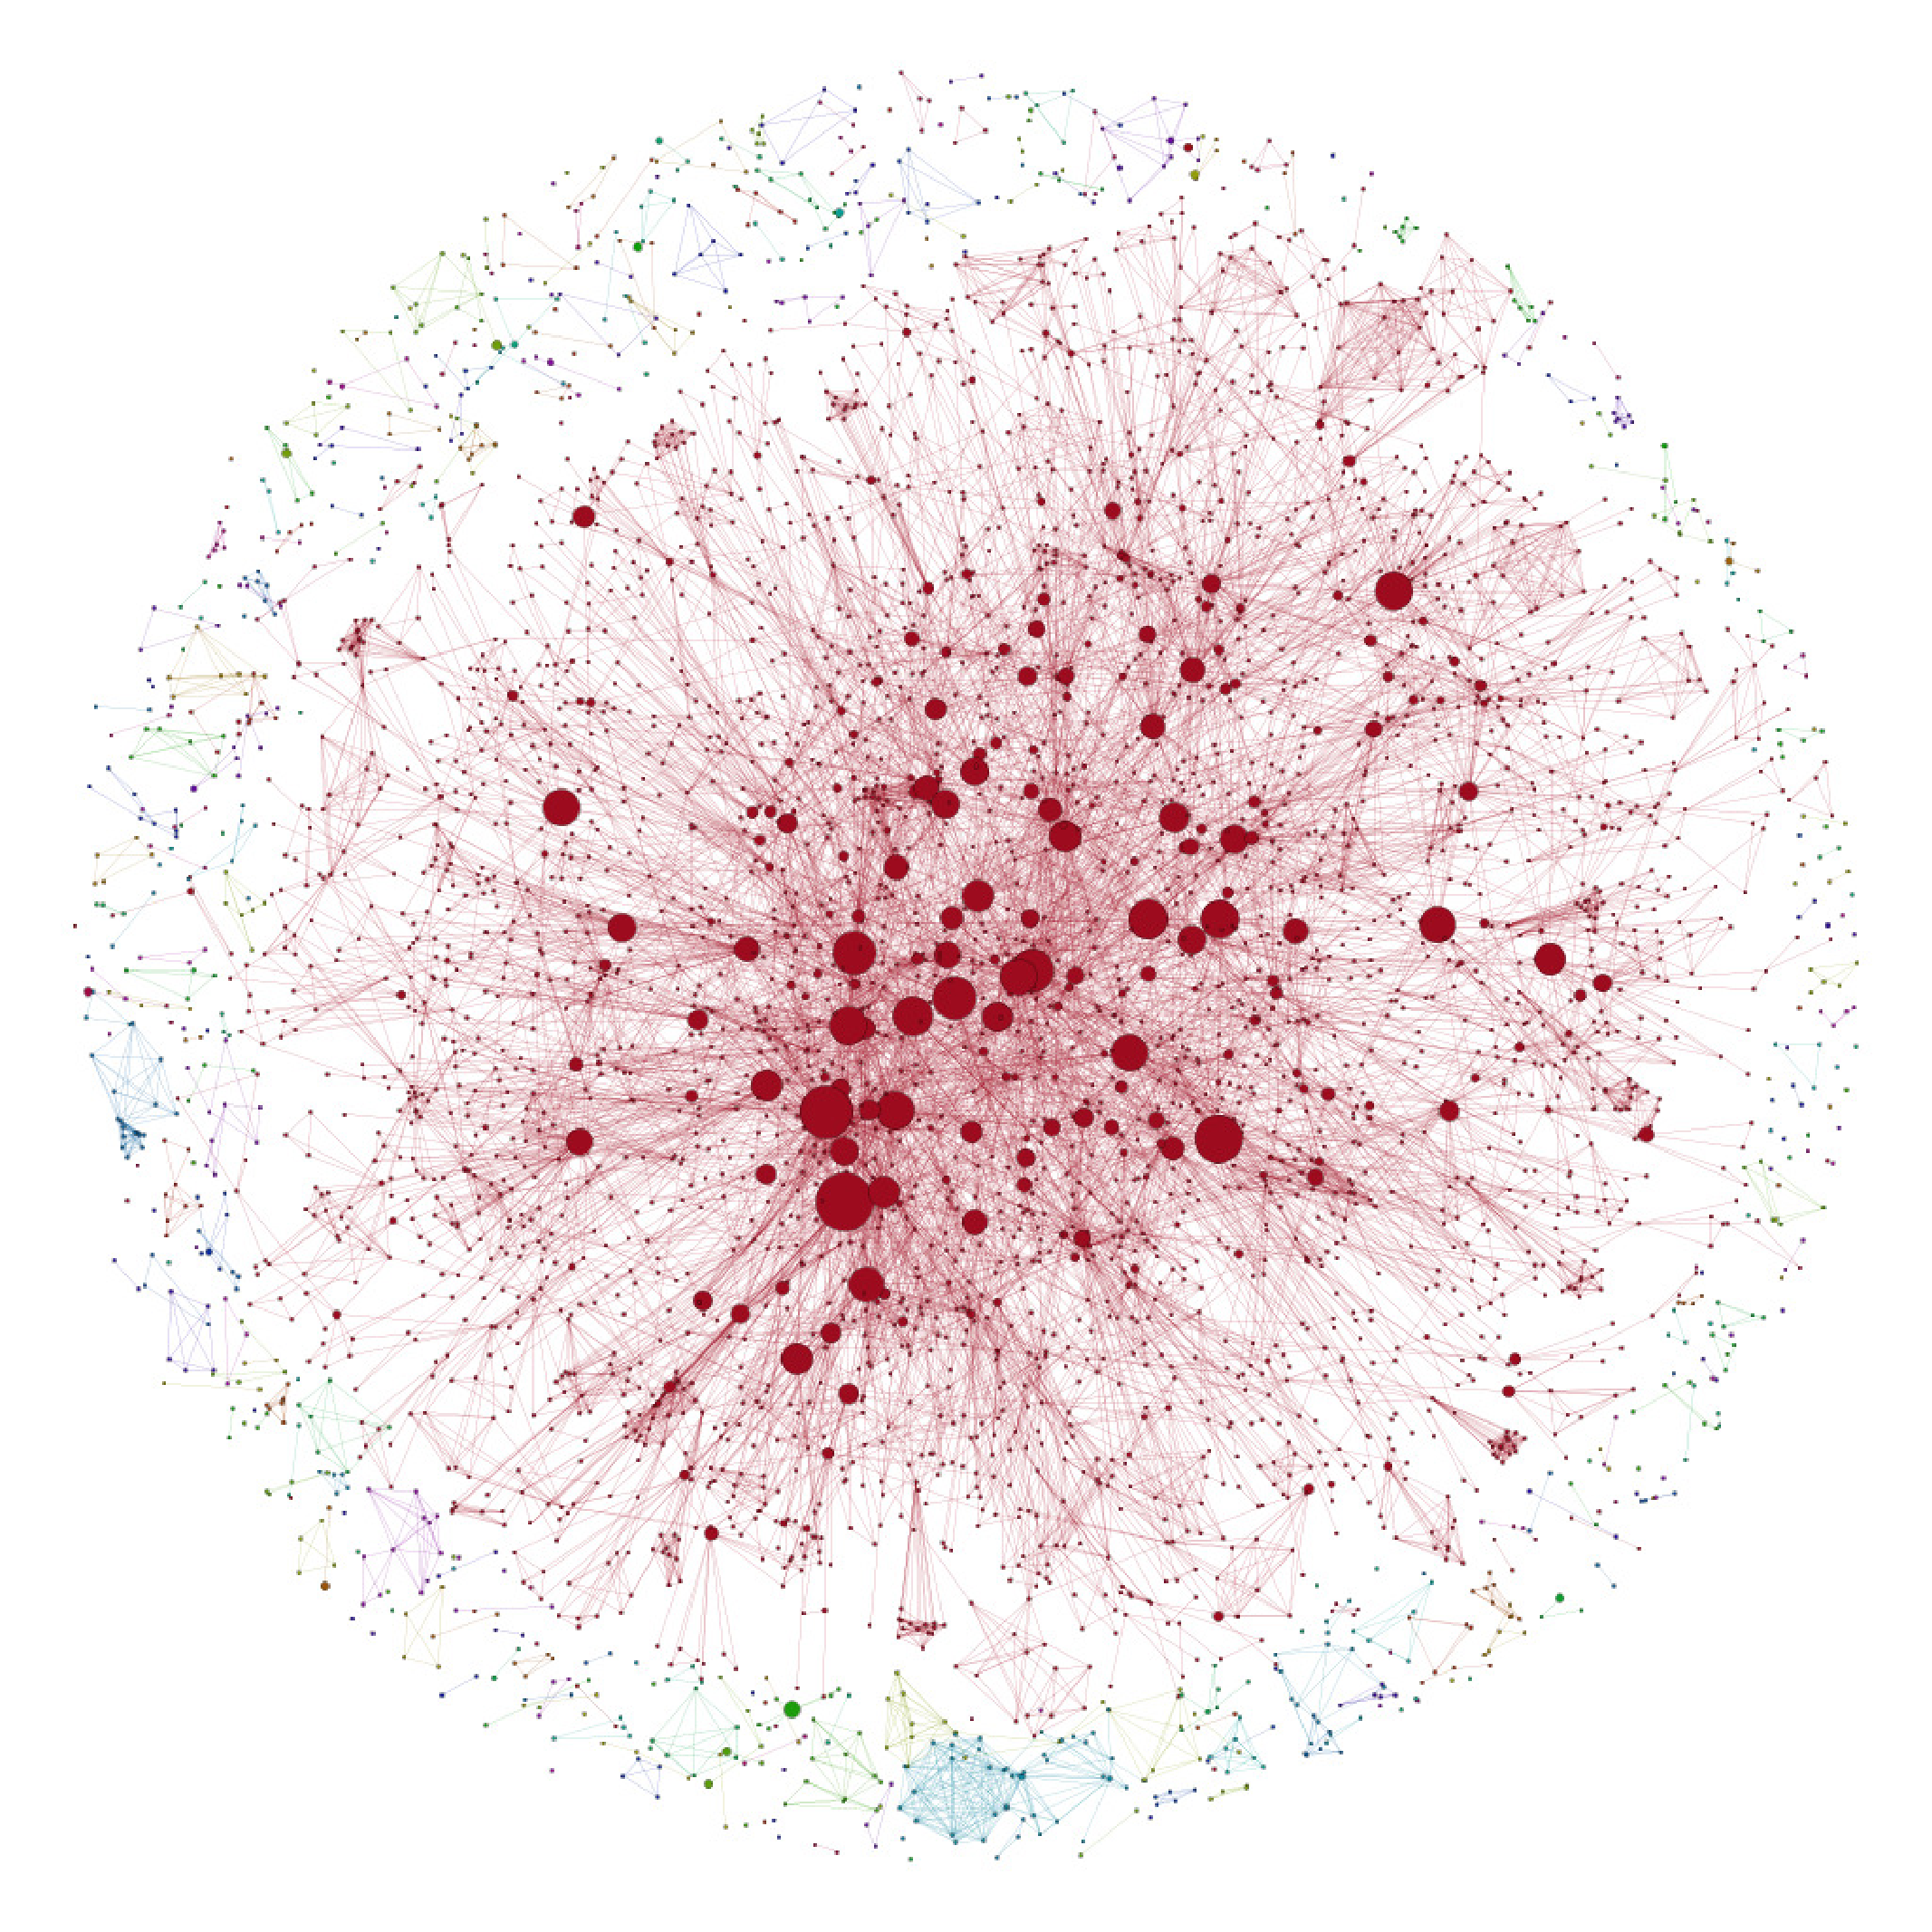
\includegraphics[scale=.135]{graficos/network/sigmod.pdf}
  }
  \subfigure[STOC (74.34\%)]{%
    \label{fig:rede_stoc}
    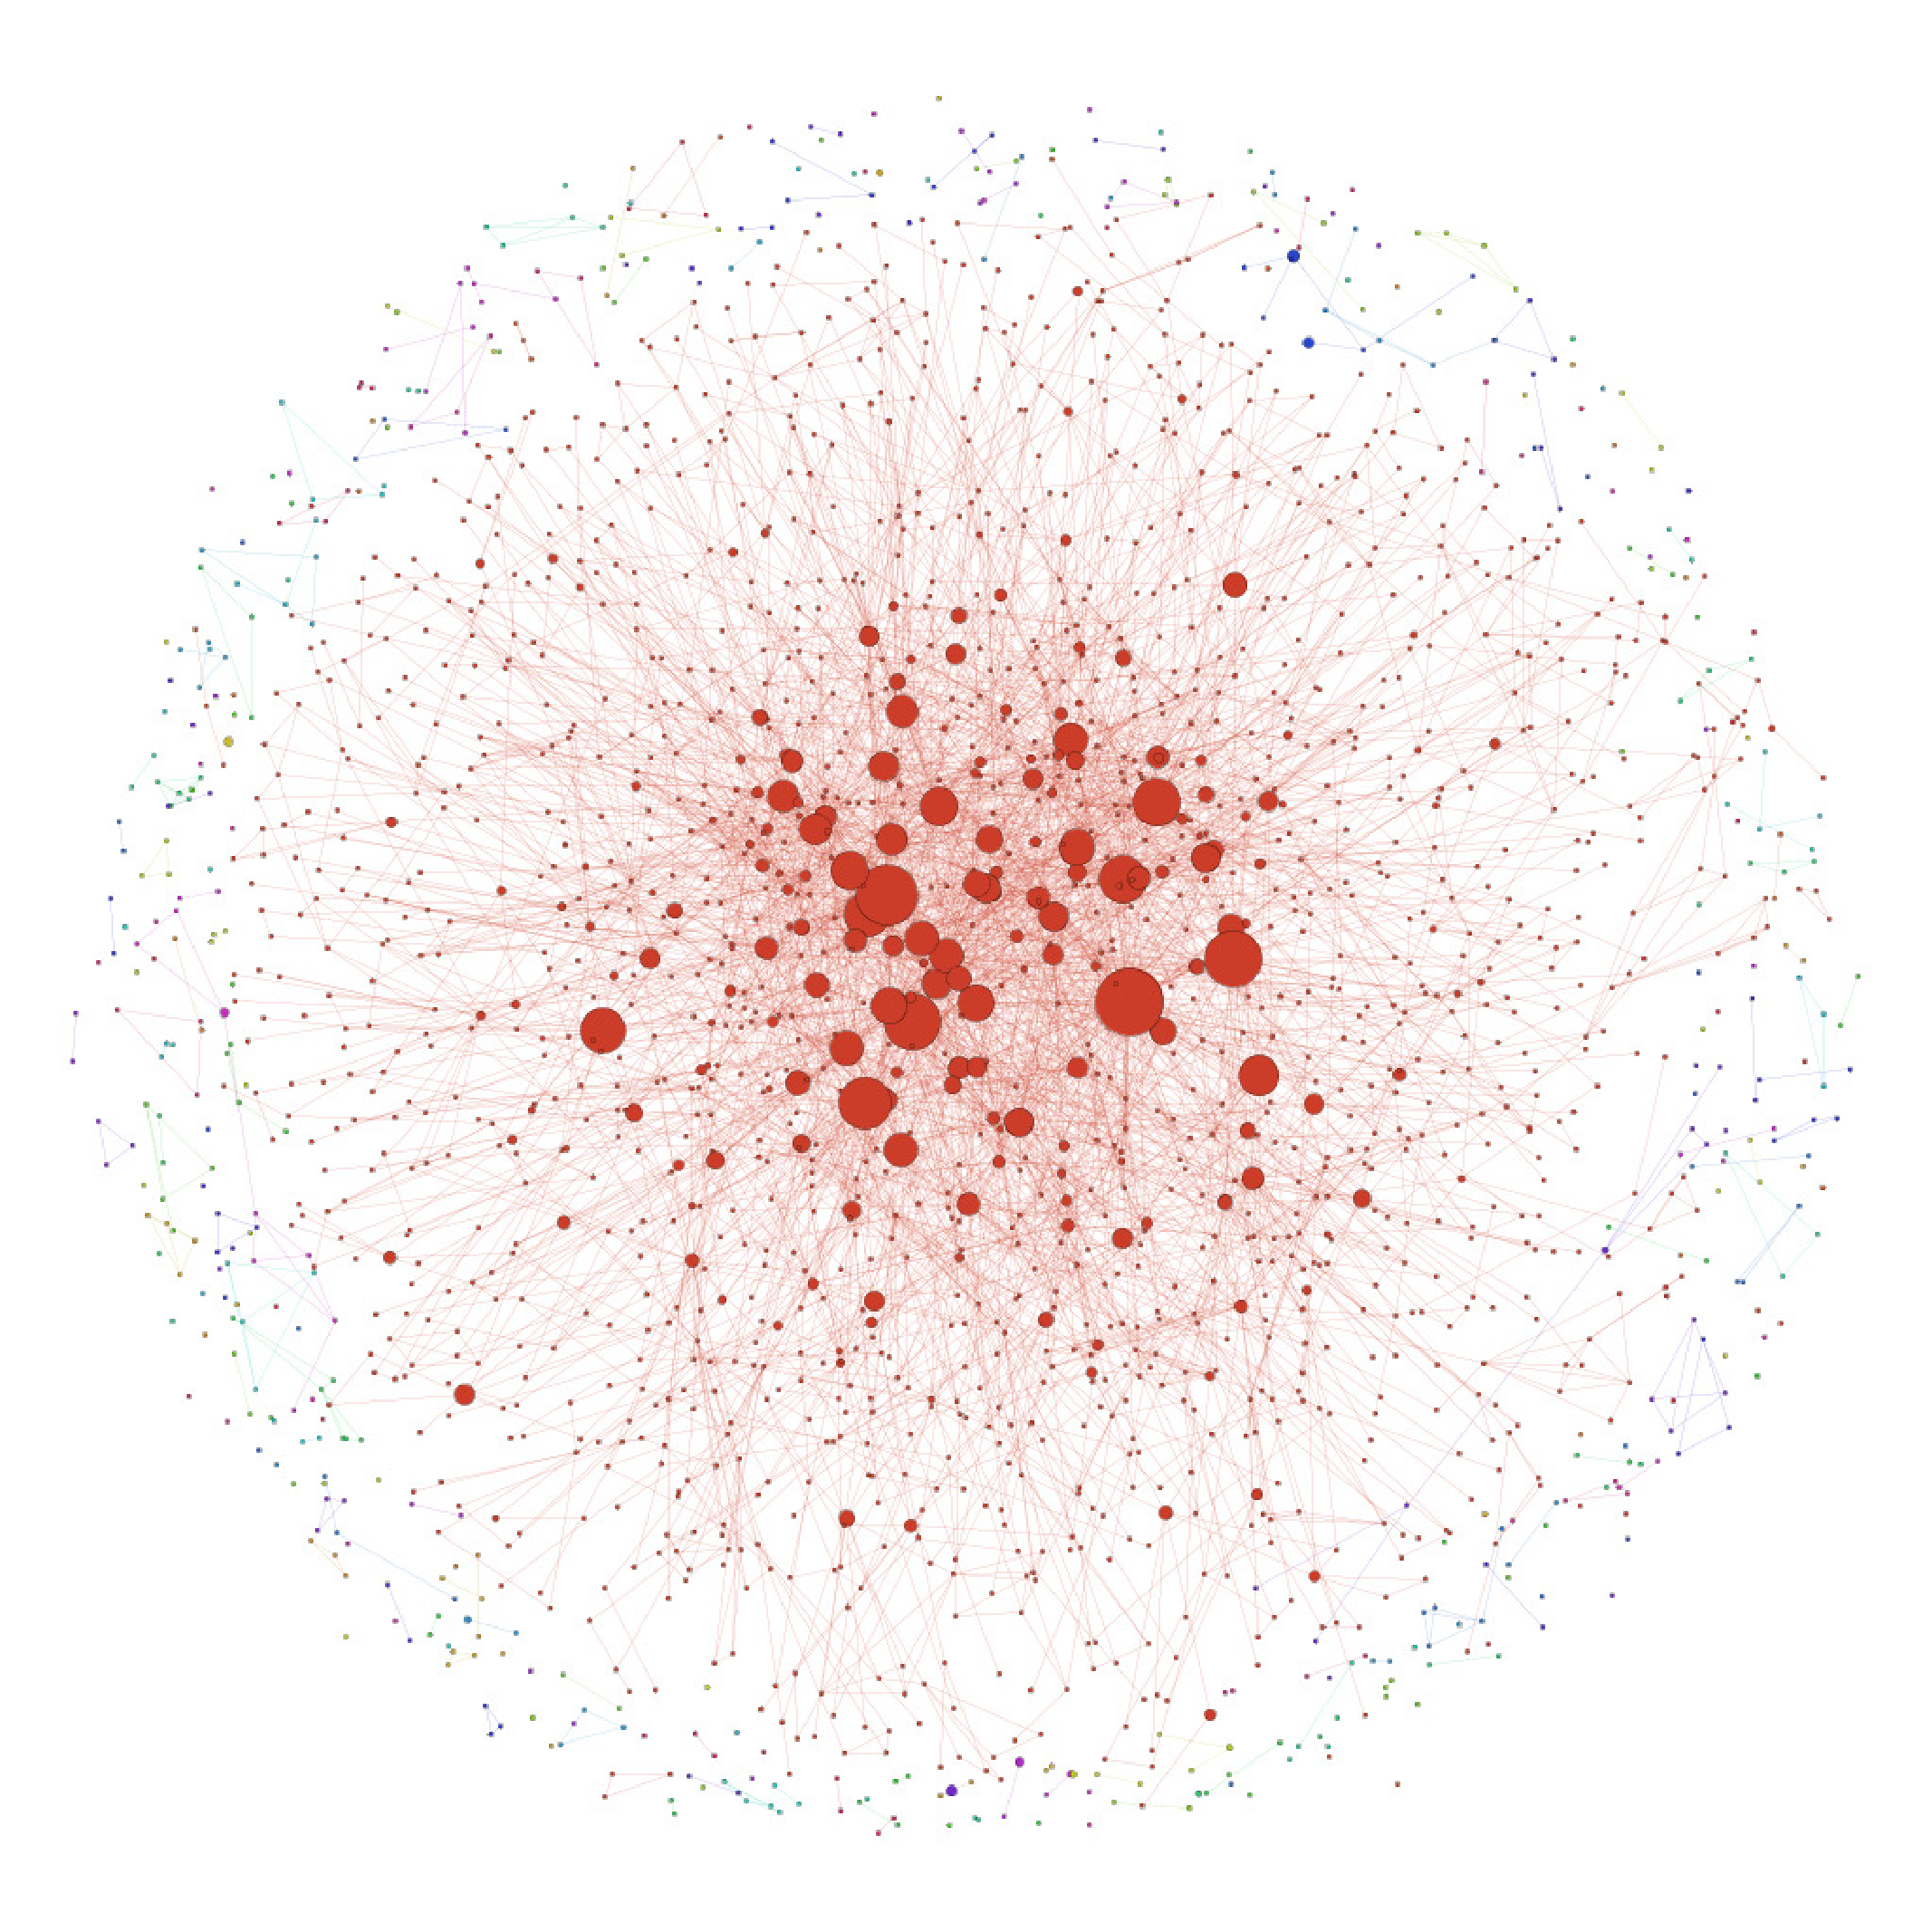
\includegraphics[scale=.135]{graficos/network/stoc.pdf}
  }
  \subfigure[CHI (73.33\%)]{%
    \label{fig:rede_chi}
    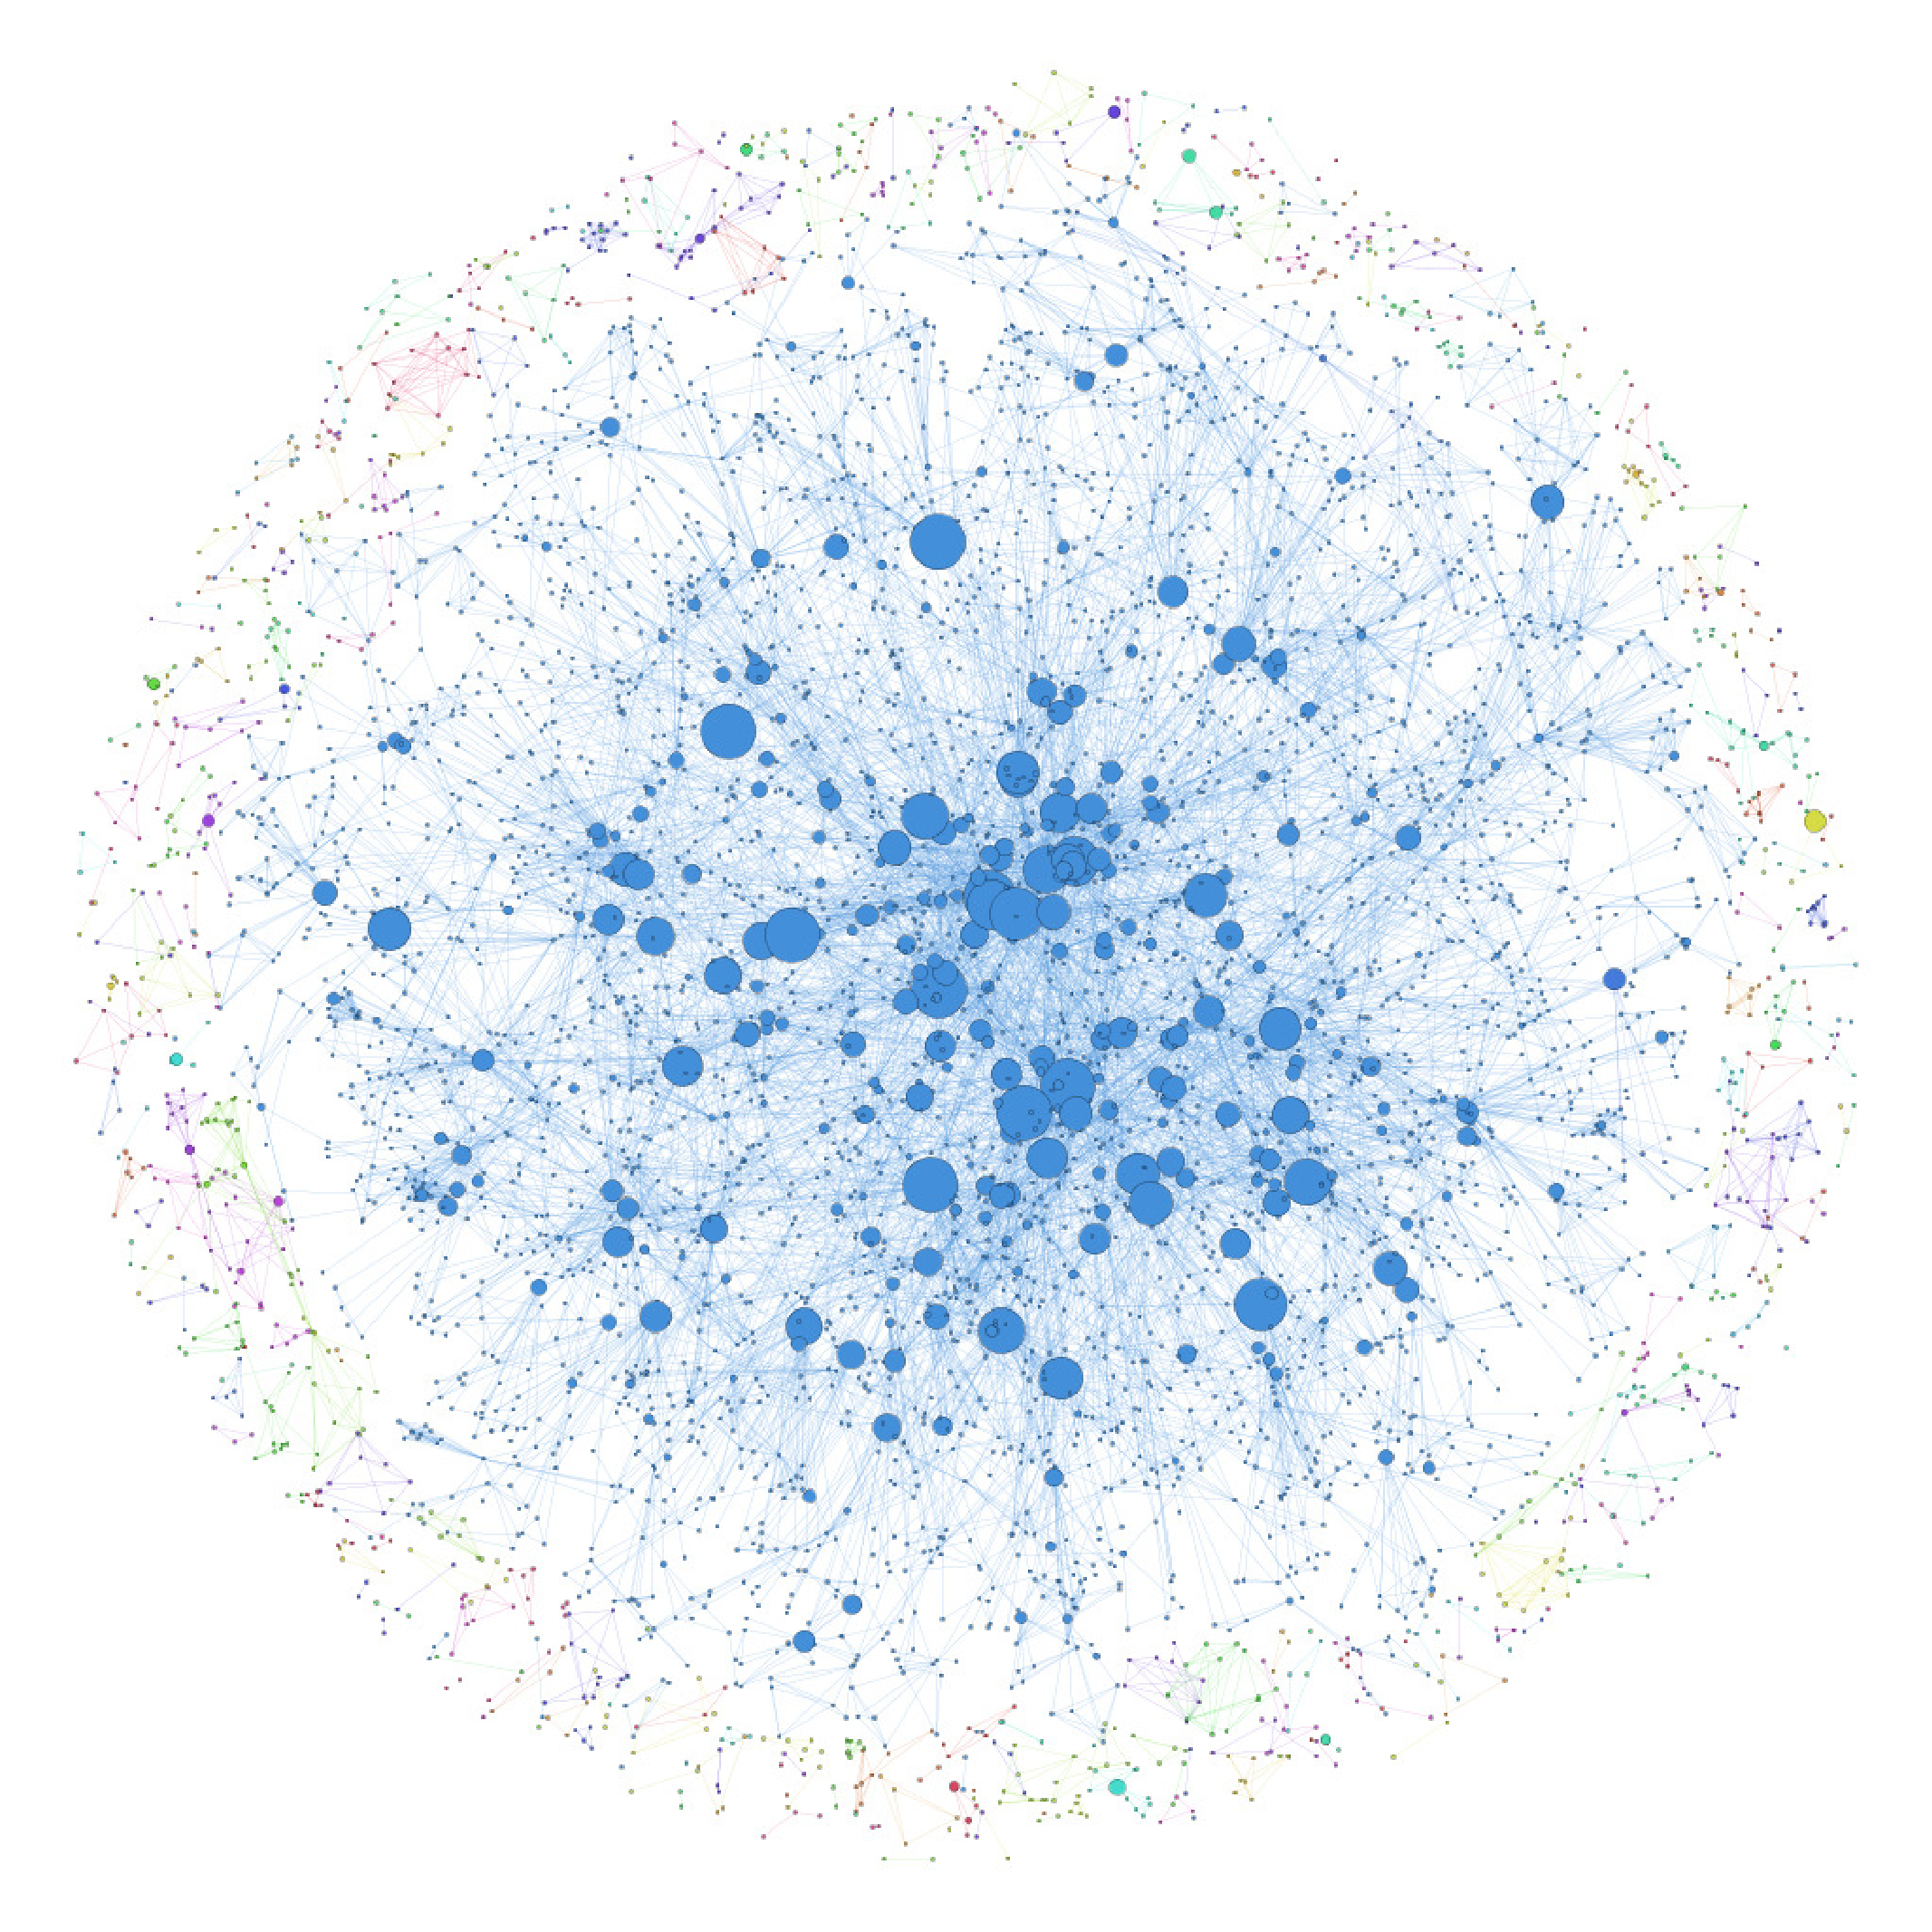
\includegraphics[scale=.135]{graficos/network/chi.pdf}
  }
    \subfigure[SIGUCCS (3.27\%)]{
    \label{fig:rede_sac}
    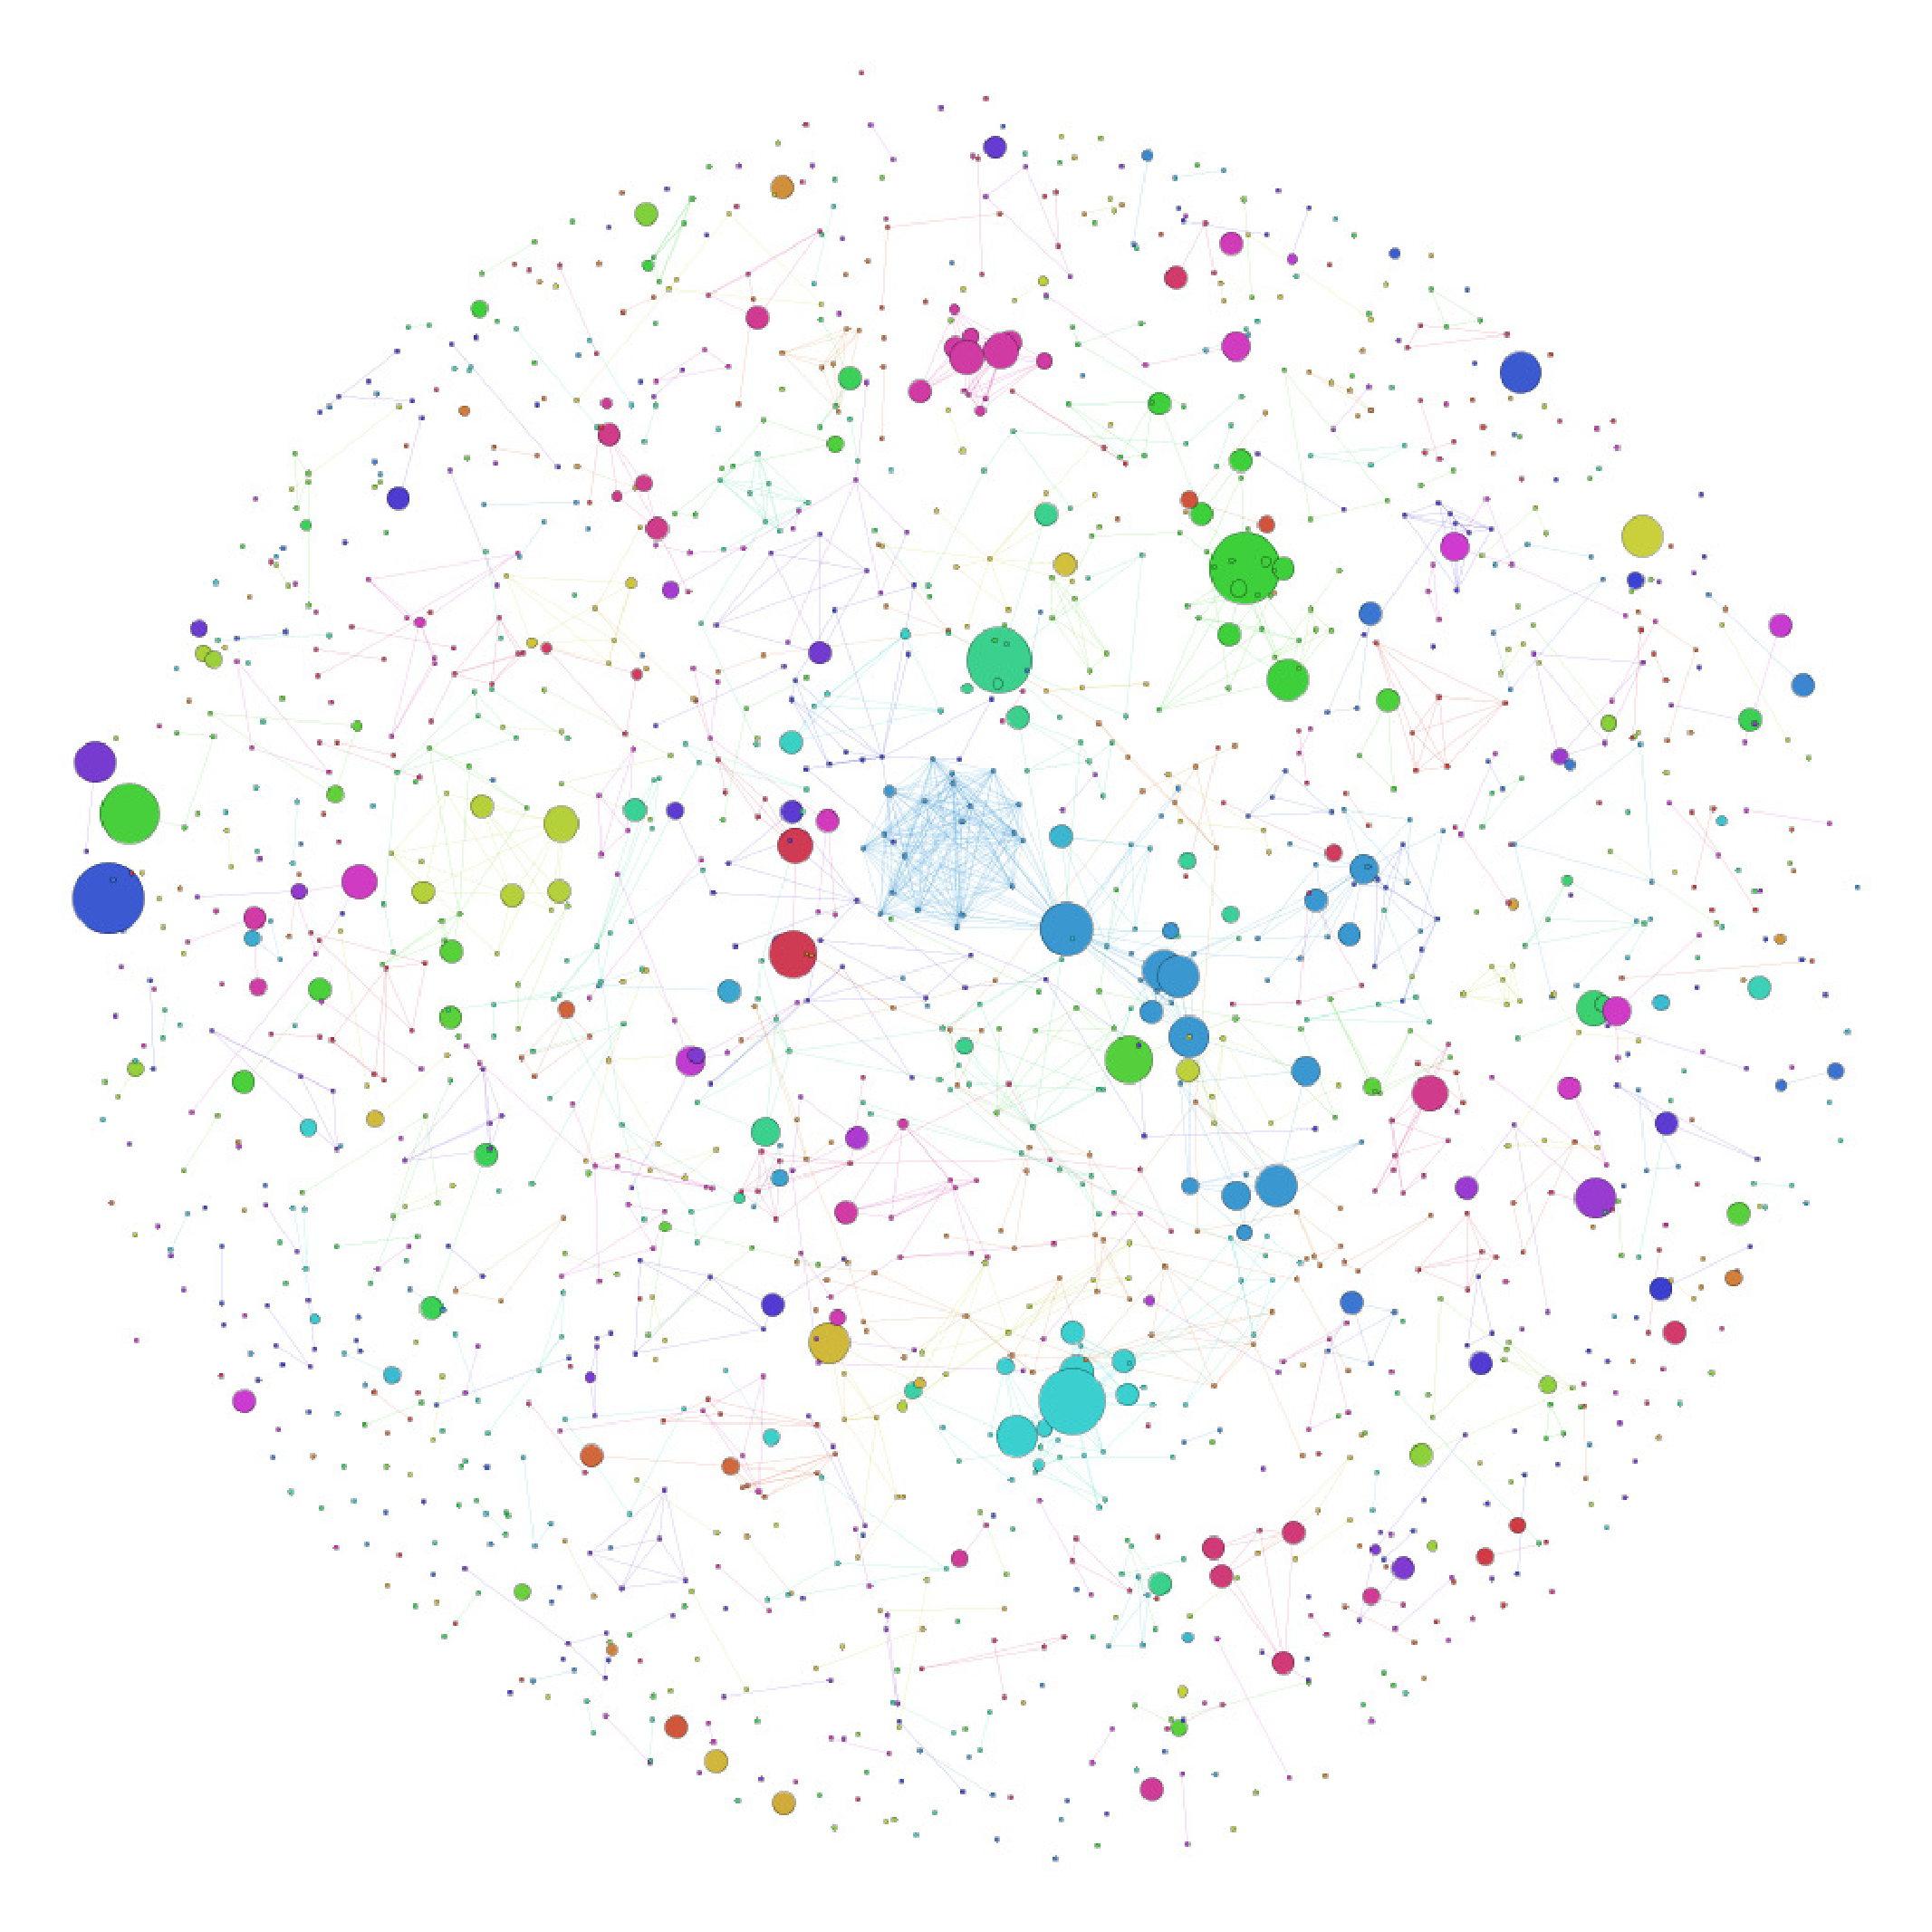
\includegraphics[scale=.135]{graficos/network/siguccs.pdf}
  }
    \subfigure[SAC (3.67\%)]{
    \label{fig:rede_sac}
    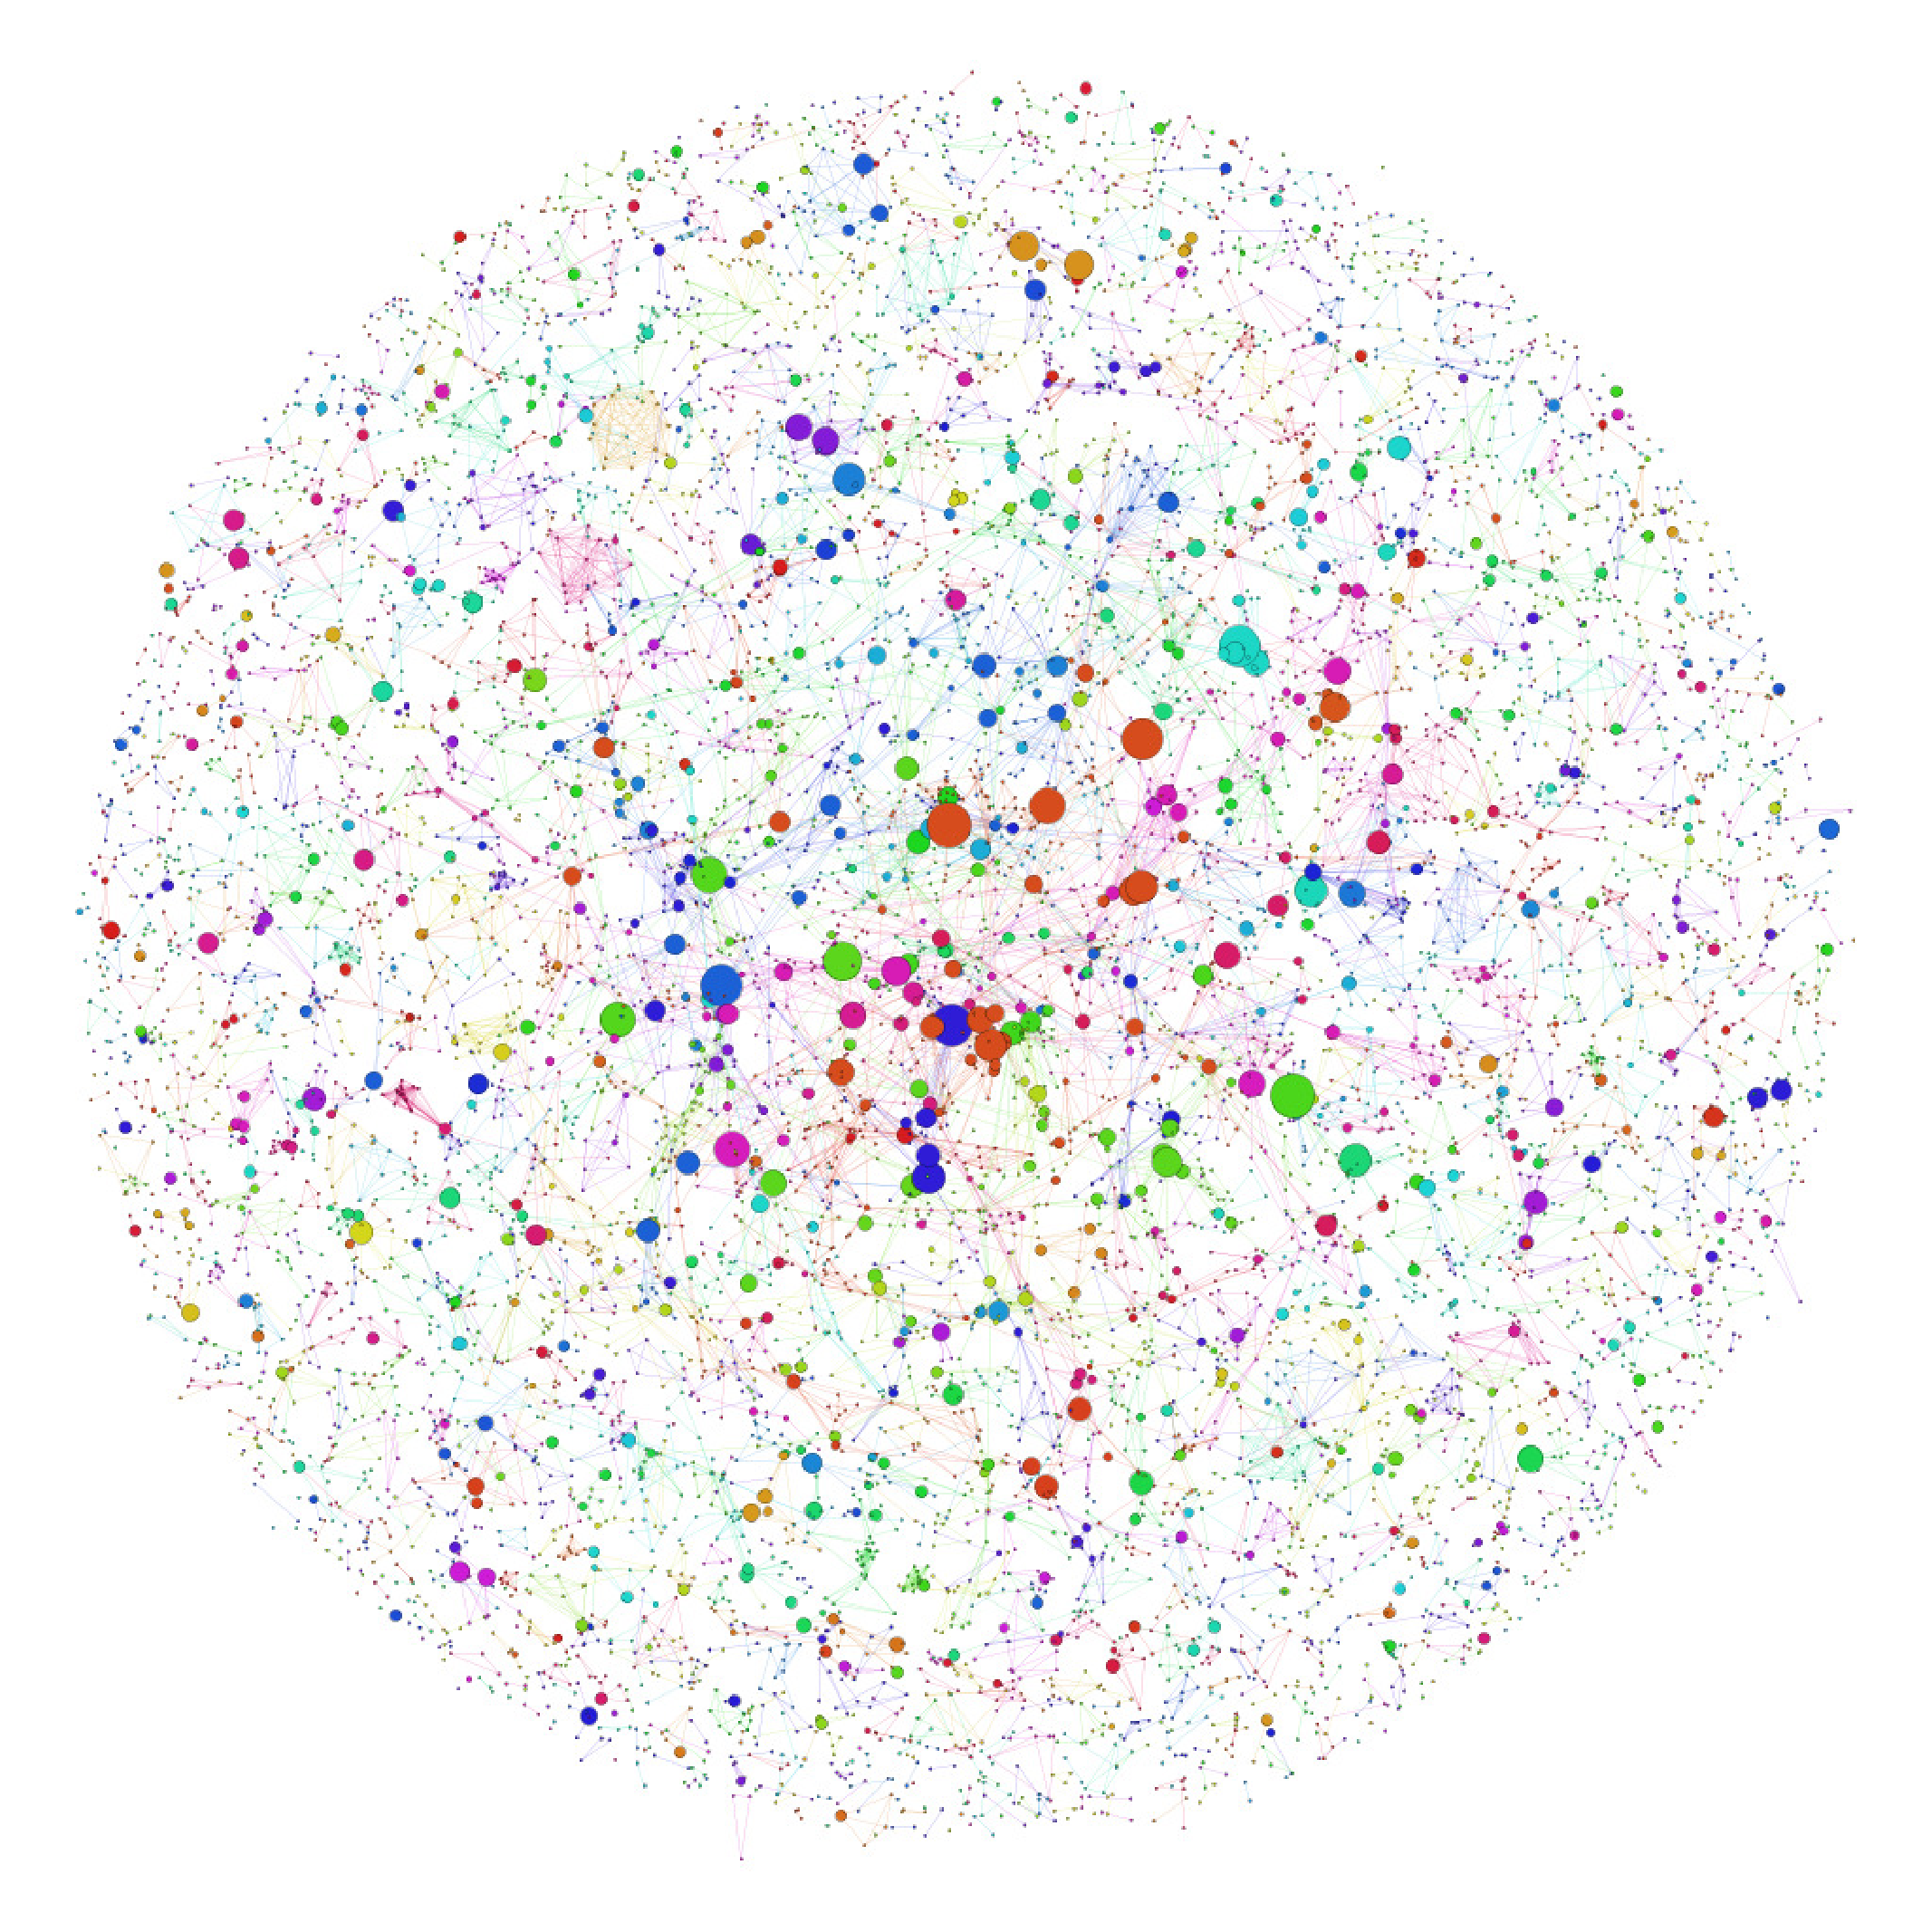
\includegraphics[scale=.135]{graficos/network/sac.pdf}
  }
  \subfigure[SIGDOC (9.69\%)]{
    \label{fig:rede_sigdoc}
    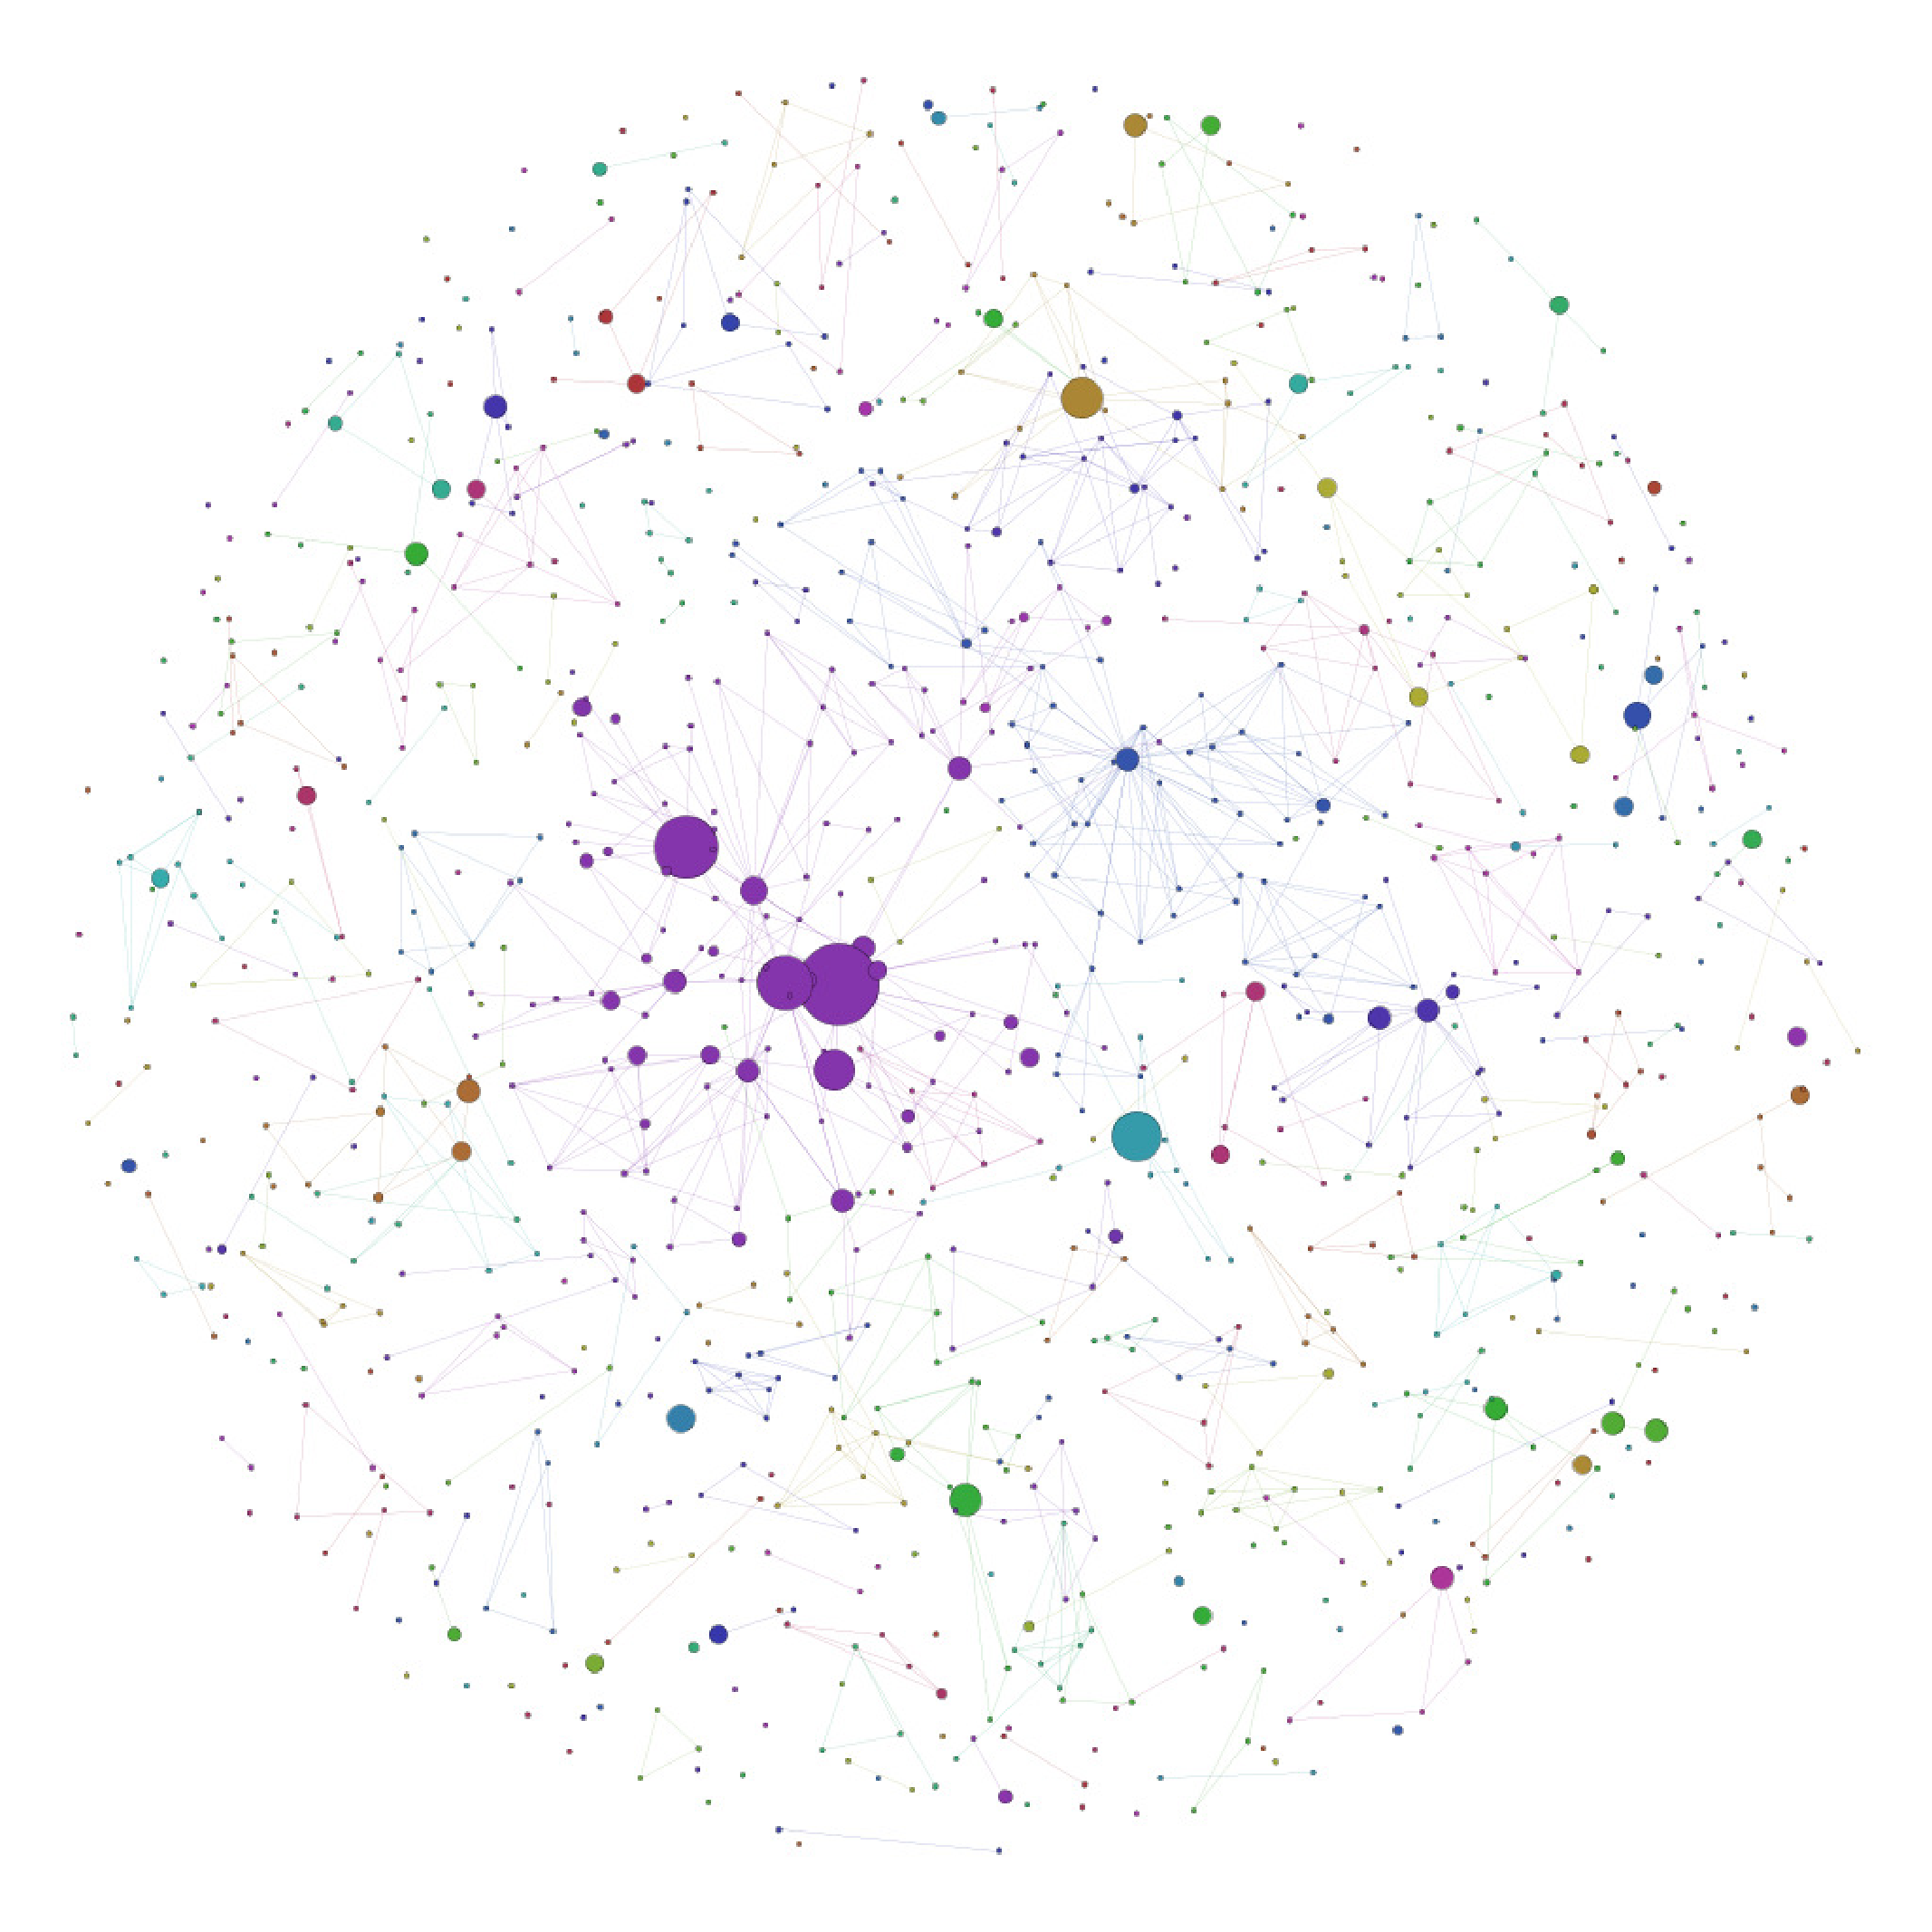
\includegraphics[scale=.135]{graficos/network/sigdoc.pdf}
  }
  \end{center}
  \caption{Scientific communities and the size of their LCC}
  \label{fig:redes_top}
\end{figure*}



\section{Leaders and Their Roles in \\Research Communities}

%Research communities have established different types of award to recognize those who were important to a certain field and helped to advance or even build a certain community.
We now turn our attention to our second research question related to identifying important members of a research community. Our intention here is not to rank researchers within their communities, but  to give a sense about which researchers have being engaged in a certain community for consecutive years and mostly helped connecting its final coauthorship graph. Thus, instead of attempting to quantify centrality measures~\cite{freeman1977set,girvan2002community} of authors and node degree in coauthorship graphs, we have defined a metric that aims at quantifying the involvement of a researcher in a scientific community in terms of publications in its flagship conference over the years. Intuitively, this metric should be able to capture (i) the prolificness of a researcher and (ii) the frequency of her involvement with a certain community. Next we discuss how exactly we have defined this metric.


\subsection{Quantifying a Researcher's \\Engagement in a Community}

First, in order to capture the prolificness of a researcher, we use the h-index~\cite{Hirsch:2005}, a metric widely adopted for this purpose. This metric consists of an index that attempts to measure both the productivity and the impact of the published work of a researcher. It is based on the set of the researcher's most cited publications and the number of citations that they have received. For example, a researcher $r$ has an h-index $h_r$ if she has at least \textit{h} publications that have received at least \textit{h} citations. Thus, for instance, if a researcher has 10 publications with at least 10 citations, her h-index is 10.

Then, as an attempt to capture the importance of a researcher to a specific community in a certain period of time, we multiply her h-index by the number of publications this researcher has in a certain community (conference) during a time window. We name this metric \textit{CoScore}, as it aims to measure the importance of a researcher as a member of the community~\cite{Alves:2013}.
More formally, the \textit{CoScore} of a researcher $r$ in a community $c$ during a period of time $t$, $Co{ }Score_{r,c,t}$, is given by her h-index $h_r$ multiplied by the number of publications $r$ has in $c$ during $t$ ($\textrm{\#}publications_{r,c,t}$), as expressed by the following equation:
\begin{equation}
  \label{eq:core_score}
  CoScore_{r,c,t} = h_r \times \textrm{\#}publications_{r,c,t}
\end{equation}

We note that the first part of the above equation captures the importance of a researcher to the scientific community as a whole regardless of any specific research area or period of time, and the second part weights this importance based on the activity of the researcher in a certain community over a period of time. The idea is to compute the amount of time a certain research appeared among the top researchers in terms of this metric over periods of a few consecutive years. For example, if a researcher that today has a high h-index has published four papers at KDD in a period of three years, it means she is engaged with that community at least for that short period of time. If a researcher appears among the top ones within a community for several of these periods, it suggests that she has a life of contributions dedicated to that community. Next, we briefly describe how we have inferred the h-index of the researchers.

%By computing the \textit{coreScore} for the members of a community, we define the community core in a certain period of time as the top researchers of that community in terms of their core scores in the given period.
%We define the community core as top 10\% researchers with highest \textit{CoreScore} values and we set time window used in our analyses for 3 years.  We refer the reader to a prior
%publication that uses the Core Score metric for justifications of its threshold choices~\cite{Alves:2013}.  Next, we briefly describe how we inferred the h-index of the researchers.


%\subsection{Inferring Researchers' H-index}
%\label{sub:hindex}

%\\
\subsection{Inferring Researchers' H-index}

There are multiple tools that measure the h-index of researchers, out of which Google Scholar Citations\footnote{http://scholar.google.com/citations} is the most prominent one. However, to have a profile in this system, a researcher needs to sign up and explicitly create her research profile. In a preliminary collection of part of the profiles of the DBLP authors, we found that less than 30\% of these authors had a profile on Google Scholar. Thus, this strategy would reduce our dataset and potentially introduce bias when analyzing the communities.

To divert from this limitation, we used data from the SHINE (Simple HINdex Estimation) project\footnote{http://shine.icomp.ufam.edu.br/} to infer the researchers' h-index. SHINE provides a website that allows users to check the h-index of almost 1800 computer science conferences. The SHINE developers crawled Google Scholar, searching for the title of papers published in these conferences, which allowed them to effectively estimate the h-index of the target conferences based on the citations computed by Google Scholar. Although SHINE only allows one to search for the h-index of conferences, the SHINE developers kindly allowed us to access their dataset to infer the h-index of researchers based on the conferences they crawled.

\begin{figure}[!htb]
\centering
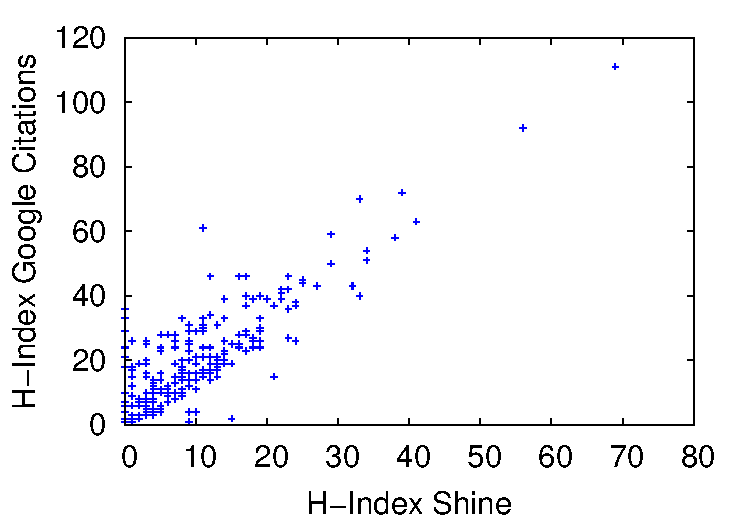
\includegraphics[scale=.45]{graficos/hindex/hindex_scatter_plot-eps-converted-to.pdf}
\caption{Correlation between the inferred h-index and Google Scholar Citations one}
\label{fig:hindex_scatter_plot}
\end{figure}

However, there is a limitation with this strategy. As SHINE does not track all existing computer science conferences, researchers' h-index might be underestimated when computed with this data. To investigate this issue, we compared the h-index of a set of researchers with a profile on Google Scholar with their estimated h-index based on the SHINE data. For this, we randomly selected 10 researchers from each conference in Table~\ref{tab:sigs_conference_period} and extracted their h-indexes from their Google Scholar profiles. 

In comparison with the h-index we estimated from SHINE, the Google Scholar values are, on average, 50\% higher.
Figure~\ref{fig:hindex_scatter_plot} shows the scatterplot for the two h-index measures. We can note that although the SHINE-based h-index is smaller, the two measures are highly correlated. The Pearson's correlation coefficient is 0.85, which indicates that researchers might have proportional h-index estimations in both systems.


\subsection{Visualizing Community Members and their Roles within the Communities}

In order to make our results public, we have developed an interactive tool\footnote{Available at \url{www.acmsig-communities.dcc.ufmg.br}} that allows one to browse the scientific communities, visualizing their structures and the contribution of each specific researcher to connect their coauthorship graph. Our effort consists in allowing users to search for researchers based on the metric presented in the previous section. The size of each author's node is proportional to the number of times she appears within the top 10\% researchers with highest \textit{CoScore} values in a time window of three years. Figure~\ref{fig:stonebraker} shows, for example, the coauthorship graph of Michael Stonebracker, the winner of the 2014 A.M. Turing Award\footnote{\url{http://amturing.acm.org/stonebraker_1172121.pdf}}, and his connections within the SIGMOD community. These connections are highlighted when one passes the mouse over the researcher's name. In addition, our tool allows one not only to search for authors but also to visualize statistics about them within the communities.


\begin{figure}[!htb]
\centering
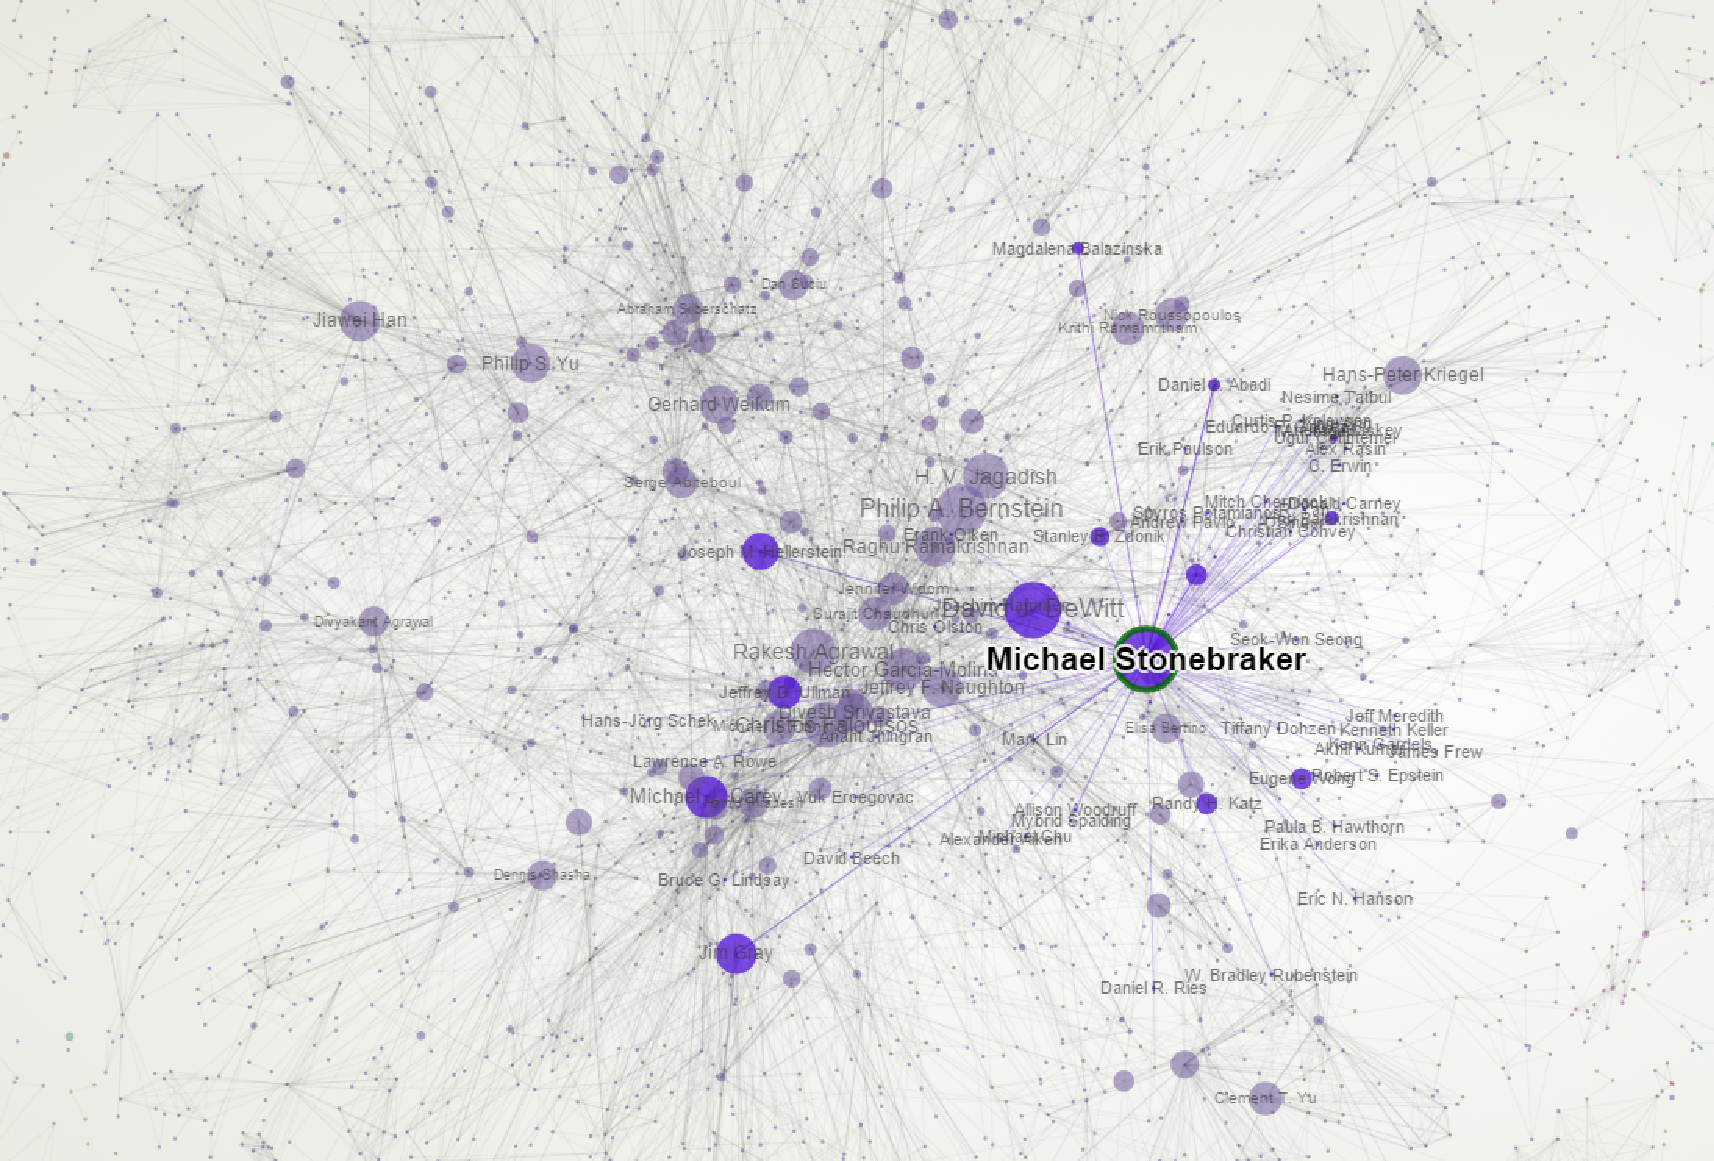
\includegraphics[scale=.28]{graficos/stonebraker.pdf}
\caption{Michael Stonebraker and his connections within the SIGMOD community}
\label{fig:stonebraker}
\end{figure}

To check if our approach really identifies  those who are prolific and engaged in a specific community,
we notice that several research communities have established different awards to recognize those who were important to a certain field and helped to advance or even build a certain community. Thus, we use some of these awards to corroborate the effectiveness of our metric in establishing the importance of a researcher within a specific community.
We have computed a ranking of the researchers that appear most often in the top 10\% of the \textit{CoScore} ranking over the years for each community. We have chosen the CHI, ICSE, KDD, POPL, SIGCOMM, SIGGRAPH, SIGIR, and SIGMOD communities to show their top 20 researchers in Tables~\ref{tab:authors_frequency_core_community1} and~\ref{tab:authors_frequency_core_community2}. As we can see, several well known names appear in these top lists, including past keynote speakers of those conferences and awardees for their life time contributions in the respective community (names in bold). In addition, besides Michael Stonebraker, these top lists include four other winners of the A.M. Turing Award (indicated by asterisks): Amir Pnueli (1996), Jim Gray (1998), Edmund M. Clarke (2007) and Barbara Liskov (2008). Indeed, by analyzing all these awardees from each community, we found that a large fraction of them appeared in the top 10\% of the \textit{CoScore} ranking at least once in the conference history. For example, according to the respective ACM SIG websites, these fractions are 75\% for KDD\footnote{http://www.sigkdd.org/awards\_innovation.php}, 35\% for SIGCOMM\footnote{http://www.sigcomm.org/awards/sigcomm-awards}, 60\% for SIGIR\footnote{http://www.sigir.org/awards/awards.html}, and 80\% for SIGMOD\footnote{http://www.sigmod.org/sigmod-awards}. Except for SIGCOMM, a community with many sponsored conferences that were not considered in our dataset, the other three communities presented very high numbers of awardee members that appear at least once in the top 10\% of the \textit{CoScore} ranking over the years.  These observations provide evidence that our approach correctly captures the notion we wanted to.


\begin{table*}[t]
\centering
\caption{Researchers that appear most often in the top 10\% of the CoScore ranking over the years}{
%\fontsize{9.2}{11}\selectfont
\begin{scriptsize}
\begin{tabular}{|c|c|c|c|} \hline
\textbf{CHI} & \textbf{ICSE} & \textbf{KDD} & \textbf{POPL}\\ \hline
\textbf{Scott E. Hudson} & \textbf{Victor R. Basili} & \textbf{Heikki Mannila} & Thomas W. Reps\\ \hline
\textbf{Hiroshi Ishii} & \textbf{Barry W. Boehm} & Hans-Peter Kriegel & Martín Abadi\\ \hline
\textbf{Steve Benford} & \textbf{Jeff Kramer} & \textbf{Jiawei Han} & John C. Mitchell\\ \hline
\textbf{George G. Robertson} & \textbf{Mary Shaw} & Martin Ester & Robert Harper\\ \hline
\textbf{Shumin Zhai} & Dewayne E. Perry & \textbf{Rakesh Agrawal} & Zohar Manna\\ \hline
\textbf{Brad A. Myers} & Don S. Batory & Bing Liu & Benjamin C. Pierce\\ \hline
\textbf{Robert E. Kraut} & Mary Jean Harrold & Ke Wang & Amir Pnueli$^\star$\\ \hline
\textbf{Elizabeth D. Mynatt} & \textbf{Lori A. Clarke} & \textbf{Padhraic Smyth} & \textbf{Barbara Liskov}$^\star$\\ \hline
\textbf{Ravin Balakrishnan} & Gruia-Catalin Roman & Philip S. Yu & Martin C. Rinard\\ \hline
\textbf{James A. Landay} & Premkumar T. Devanbu & Charu C. Aggarwal & Luca Cardelli\\ \hline
Ken Hinckley & Gail C. Murphy & \textbf{Vipin Kumar} & Thomas A. Henzinger\\ \hline
\textbf{Mary Czerwinski} & \textbf{Richard N. Taylor} & Wynne Hsu & \textbf{Ken Kennedy}\\ \hline
\textbf{Carl Gutwin} & \textbf{David Garlan} & Qiang Yang & \textbf{Matthias Felleisen}\\ \hline
\textbf{Gregory D. Abowd} & Michael D. Ernst & \textbf{Christos Faloutsos} & Edmund M. Clarke$^\star$\\ \hline
Michael J. Muller & James D. Herbsleb & William W. Cohen & Mitchell Wand\\ \hline
\textbf{Susan T. Dumais} & Lionel C. Briand & Pedro Domingos & David Walker\\ \hline
Loren G. Terveen & Gregg Rothermel & Eamonn J. Keogh & Simon L. Peyton Jones\\ \hline
\textbf{Steve Whittaker} & Kevin J. Sullivan & Alexander Tuzhilin & Shmuel Sagiv\\ \hline
W. Keith Edwards & \textbf{David Notkin} & Mohammed Javeed Zaki & Barbara G. Ryder\\ \hline
\textbf{John M. Carroll} & Douglas C. Schmidt & Mong-Li Lee & Alexander Aiken\\ \hline
\end{tabular}
\end{scriptsize}
% \par\medskip\footnotesize{$^\star$ Pesquisadores premiados por uma vida de inovação e liderança dentro daquela comunidade.}
% \par\medskip\footnotesize{$^\star$ Pesquisadores agraciados com \textit{A. M. Turing Award}.}
}
\label{tab:authors_frequency_core_community1}
\end{table*}


\begin{table*}[t]
\centering
\caption{Researchers that appear most often in the top 10\% of the CoScore ranking over the years}
%\fontsize{9.2}{11}\selectfont
\begin{scriptsize}
\begin{tabular}{|c|c|c|c|} \hline
\textbf{SIGCOMM} & \textbf{SIGGRAPH} & \textbf{SIGIR} & \textbf{SIGMOD}\\ \hline
\textbf{Scott Shenker} & \textbf{Donald P. Greenberg} & \textbf{W. Bruce Croft} & \textbf{Michael Stonebraker}$^\star$\\ \hline
George Varghese & \textbf{Pat Hanrahan} & Clement T. Yu & \textbf{David J. DeWitt}\\ \hline
\textbf{Donald F. Towsley} & Demetri Terzopoulos & \textbf{Gerard Salton} & \textbf{Philip A. Bernstein}\\ \hline
Ion Stoica & \textbf{David Salesin} & Alistair Moffat & H. V. Jagadish\\ \hline
Hui Zhang & \textbf{Michael F. Cohen} & \textbf{Susan T. Dumais} & Christos Faloutsos\\ \hline
Deborah Estrin & \textbf{Richard Szeliski} & James Allan & \textbf{Rakesh Agrawal}\\ \hline
Hari Balakrishnan & John F. Hughes & Yiming Yang & \textbf{Michael J. Carey}\\ \hline
Robert Morris & N. Magnenat-Thalmann & Edward A. Fox & \textbf{H. Garcia-Molina}\\ \hline
Thomas E. Anderson & \textbf{Tomoyuki Nishita} & James P. Callan & Jiawei Han\\ \hline
Ramesh Govindan & \textbf{Andrew P. Witkin} & Chris Buckley & Raghu Ramakrishnan\\ \hline
Srinivasan Seshan & Norman I. Badler & \textbf{C. J. van Rijsbergen} & Jeffrey F. Naughton\\ \hline
David Wetherall & \textbf{Peter Schröder} & Justin Zobel & \textbf{Jim Gray}$^\star$\\ \hline
Yin Zhang & Steven Feiner & Ellen M. Voorhees & Hans-Peter Kriegel\\ \hline
Jennifer Rexford & \textbf{Hugues Hoppe} & Mark Sanderson & Gerhard Weikum\\ \hline
Jia Wang & \textbf{Jessica K. Hodgins} & \textbf{Norbert Fuhr} & Philip S. Yu\\ \hline
J. J. Garcia-Luna-Aceves & \textbf{Greg Turk} & Nicholas J. Belkin & Divesh Srivastava\\ \hline
Randy H. Katz & \textbf{Marc Levoy} & Chengxiang Zhai & Joseph M. Hellerstein\\ \hline
Albert G. Greenberg & \textbf{P. Prusinkiewicz} & Charles L. A. Clarke & Krithi Ramamritham\\ \hline
Mark Handley & Eihachiro Nakamae & Alan F. Smeaton & Nick Roussopoulos\\ \hline
\textbf{Simon S. Lam} & Dimitris N. Metaxas & Gordon V. Cormack & \textbf{Surajit Chaudhuri}\\ \hline
\end{tabular}
\label{tab:authors_frequency_core_community2}
\end{scriptsize}
% \par\medskip\footnotesize{$^\star$ Pesquisadores premiados por uma vida de inovação e liderança dentro daquela comunidade.}
% \par\medskip\footnotesize{$^\star$ Pesquisadores agraciados com \textit{A. M. Turing Award}.}
\end{table*}



\section{Conclusions}

This work analyzes the structure of the communities formed by the flagship conferences of ACM SIGs. Our findings show that most of the ACM SIGs are able to connect their main authors in large and visually well-structured communities. However, we note that a few conferences, such as the ACM Symposium on Applied Computing, flagship conference of SIGAPP, and the ACM Conference on Design of Communications, flagship conference of SIGDOC, do not form a strong research community, presenting a structure with several disconnected components. We have opened our results to the research community as an interactive visualization tool that allows one to browse the scientific communities, visualizing their structures and the contribution of each specific researcher to connect its coauthorship graph.


\section*{Acknowledgments}

This work was partially funded by InWeb - The Brazilian National Institute
of Science and Technology for the Web (grant MCT/CNPq 573871/2008-6), and
by the authors' individual grants from CNPq, CAPES e FAPEMIG.



\bibliographystyle{abbrv}

%\small{
\begin{thebibliography}{10}
\vspace{0.1cm}
\bibitem{Alves:2013}
B.~L. Alves, F.~Benevenuto, and A.~H.~F. Laender.
\newblock {The Role of Research Leaders on the Evolution of Scientific
  Communities}.
\newblock In {\em Proceedings of the 22nd International Conference on World
  Wide Web (Companion Volume)}, pages 649--656, 2013.

\bibitem{benevenuto2015hindexparadox}
F.~Benevenuto, A.~H.~F. Laender, and B.~L. Alves.
\newblock {The H-index paradox: your coauthors have a higher H-index than you
  do}.
\newblock {\em Scientometrics}, 2016 (to appear).

\bibitem{Fortnow:cacm2009}
L.~Fortnow.
\newblock {Time for Computer Science to Grow Up}.
\newblock {\em Commun. ACM}, 52(8):33--35, Aug. 2009.

\bibitem{Franceschet:cacm2010}
M.~Franceschet.
\newblock {The Role of Conference Publications in CS}.
\newblock {\em Commun. ACM}, 53(12):129--132, Dec. 2010.

\bibitem{freeman1977set}
L.~C. Freeman.
\newblock A set of measures of centrality based on betweenness.
\newblock {\em Sociometry}, pages 35--41, 1977.

\bibitem{Freyne:cacm2010}
J.~Freyne, L.~Coyle, B.~Smyth, and P.~Cunningham.
\newblock {Relative Status of Journal and Conference Publications in Computer
  Science}.
\newblock {\em Commun. ACM}, 53(11):124--132, Nov. 2010.

\bibitem{girvan2002community}
M.~Girvan and M.~E. Newman.
\newblock Community structure in social and biological networks.
\newblock {\em Proceedings of the National Academy of Sciences of the United
  States of America}, 99(12):7821--7826, 2002.

\bibitem{Hirsch:2005}
J.~E. Hirsch.
\newblock An index to quantify an individual's scientific research output.
\newblock {\em Proceedings of the National Academy of Sciences of the United
  States of America}, 102(46):16569--16572, 2005.

\bibitem{Laender:sigcse2008}
A.~H.~F. Laender, C.~J.~P. de~Lucena, J.~C. Maldonado, E.~de~Souza~e Silva, and
  N.~Ziviani.
\newblock {Assessing the Research and Education Quality of the Top Brazilian
  Computer Science Graduate Programs}.
\newblock {\em {SIGCSE} Bulletin}, 40(2):135--145, 2008.

\bibitem{Ley:2002}
M.~Ley.
\newblock {The {DBLP} Computer Science Bibliography: Evolution, Research
  Issues, Perspectives}.
\newblock In {\em Proceedings of the 9th International Symposium on String
  Processing and Information Retrieval}, pages 1--10, 2002.

\bibitem{Ley:2009}
M.~Ley.
\newblock {DBLP: Some Lessons Learned}.
\newblock {\em Proc. of VLDB Endow.}, 2(2):1493--1500, Aug. 2009.

\bibitem{newman2010networks}
M.~Newman.
\newblock {\em {Networks: An Introduction}}.
\newblock Oxford University Press, 2010.

\bibitem{Patterson:cacm2004}
D.~A. Patterson.
\newblock {The Health of Research Conferences and the Dearth of Big Idea
  Papers}.
\newblock {\em Commun. ACM}, 47(12):23--24, Mar. 2004.

\bibitem{Vardi:cacm2009}
M.~Y. Vardi.
\newblock {Conferences vs. Journals in Computing Research}.
\newblock {\em Commun. ACM}, 52(5):5--5, May 2009.

\bibitem{Vardi:cacm2010}
M.~Y. Vardi.
\newblock {Revisiting the Publication Culture in Computing Research}.
\newblock {\em Commun. ACM}, 53(3):5--5, Mar. 2010.

\bibitem{Vardi:cacm2014}
M.~Y. Vardi.
\newblock {Scalable Conferences}.
\newblock {\em Commun. ACM}, 57(1):5--5, Jan. 2014.

\end{thebibliography}
%}



%\\
%{\small \bibliography{references}}
%\bibliography{references}

\end{document}
